\documentclass[11pt,a4paper,openright,twoside]{book}
\def\myauthor{Adrià Arrufat}
\def\mytitle{Multiple transforms for video coding}
\usepackage[british]{babel}
\usepackage{geometry}
\geometry{verbose,tmargin=2.5cm,bmargin=2.5cm,lmargin=2.5cm,rmargin=2.5cm}
\usepackage[nottoc]{tocbibind} % see http://www.howtotex.com/packages/how-to-add-bibliography-and-more-to-table-of-contents/
\usepackage{titlesec,titletoc} % to modify titles and add partial tocs
\usepackage[printonlyused,withpage]{acronym} % options: printonlyused, withpage
\usepackage{imakeidx} % allows customizing the index in the makeindex command
\usepackage{emptypage} % removes headers and footers from empty pages
\usepackage[thickqspace,amssymb,noams]{SIunits} % consistent units support
\usepackage{subfig}
\usepackage{nicefrac}
\usepackage{contour} % for inexisting bold symbols
\usepackage{enumitem} % for custom labels
\usepackage{algorithm2e}
\usepackage{multirow}
\usepackage{tabularx}
\contourlength{0.01em}

\usepackage{color}
\definecolor{yellowish}{rgb}{1,1,0.5}
\definecolor{redish}{rgb}{1,0.25,0.25}
\providecommand{\todo}[1]{
	\begin{center}
		\colorbox{yellowish}{
			\begin{minipage}{0.95\linewidth}
				\textbf{\color{redish}{TODO}:} #1
			\end{minipage}
		}
	\end{center}
}

% lines and paragraphs
% \usepackage{setspace}
% \setstretch{1}
% \parskip=\smallskipamount
% \setlength{\parindent}{0pt}

% font configuration
\usepackage{amsmath, amssymb}
\usepackage[T1]{fontenc}
\usepackage{mathptmx}
\usepackage[scaled]{helvet}
\usepackage{courier}

\usepackage[usenames,dvipsnames]{xcolor}
\usepackage{pgfplots,tikz}
\usetikzlibrary{shapes,arrows,fit,calc,decorations.markings,intersections}
\usepgfplotslibrary{fillbetween}
\usepackage{bookmark} % needed for \bookmarksetup{startatroot}
\usepackage{hyperref}
\hypersetup{
	unicode=true,
	pdfencoding=auto,
	colorlinks=true,
	citecolor=blue,
	filecolor=red,
	linkcolor=Blue,
	urlcolor=blue,
	linktoc=all,
	pdfauthor={\myauthor},
	pdftitle={\mytitle},
	pdfsubject={video coding},
	pdfkeywords={video, image, transform},
	pdfinfo={
		CreationDate={D:20150121111947},
		%ModDate={...}
	},
}
% \urlstyle{same} % do not use monospaced fonts in urls

% Define a partial ToC to use at the beginning of every chapter
\providecommand{\chaptertoc}{
	\startcontents[chapters]
	\hrule
	\vspace{1em}
	\printcontents[chapters]{}{1}{{\bf\large Contents}}
	\hrule
}

% import mathematical and colour definitions
% mathematical definitions for convenience
\def\A{\mathbf{A}}   % transform \A
\def\a{\mathbf{a}}   % rows of transform \A
\def\C{\mathbf{C}}   % covariance matrix
\def\E{\text{E}}     % expected value
\def\I{\mathbf{I}}   % identity matrix
\def\P{\text{P}}     % probability
\def\R{\mathbf{R}}   % correlation matrix
\def\U{\mathbf{U}}   % Right SVD decomposition
\def\V{\mathbf{V}}   % Left SVD decomposition
\def\X{\mathbf{X}}   % x in the transformed domain
\def\Y{\mathbf{Y}}   % helper cross correlation matrix
\def\arg{\text{arg}} % argument
\def\c{\mathbf{c}}   % quantised coefficients
\def\d{\text{d}}     % differential
\def\e{\text{e}}     % Euler's constant
\def\GGD{\text{GGD}} % general Gaussian distribution
\def\tr{\text{tr}}   % trace
\def\x{\mathbf{x}}   % x vector
\def\Lambdab{\contour[3]{black}{$\Lambda$}} % eigen values matrix

% custom colours
\definecolor{mygreen}{RGB}{0,143,0}


\numberwithin{equation}{section} % equations referred to sections
\numberwithin{figure}{section} % figures referred to sections
\numberwithin{table}{section} % tables referred to sections

\makeindex[options=-s index-alph-group.ist]

\title{\Huge\bf\mytitle}
\author{\myauthor}

\begin{document}
\frontmatter
\maketitle

\chapter*{Acknowledgements}
\label{cha:acknowledgements}
\addcontentsline{toc}{chapter}{Acknowledgements}

% \setcounter{tocdepth}{5}
\tableofcontents
\addcontentsline{toc}{chapter}{Contents}
\cleardoublepage
\chapter*{List of Acronyms}
\label{cha:glossary}
\addcontentsline{toc}{chapter}{List of Acronyms}
\begin{acronym}[JCT-VC] % the option corresponds to the longest acronym
	\acro{AI}{All Intra}
	\acro{AR}{Auto-Regressive}
	\acro{AVC}{Advanced Video Coding}
	\acro{BD}{Bj{\o}ntegaard Delta}
	\acro{CABAC}{Context Adaptive Binary Arithmetic Coding}
	\acro{CE}{Core Experiment}
	\acro{CTC}{Common Test Conditions}
	\acro{DCT}{Discrete Cosine Transform}
	\acro{DPCM}{Differential Pulse-Code Modulation}
	\acro{DST}{Discrete Sine Transform}
	\acro{DTT}{Discrete Trigonometric Transform}
	\acro{GGD}{Generalised Gaussian Distribution}
	\acro{GOP}{Group of Pictures}
	\acroplural{GOP}[GOPs]{Groups of Pictures}
	\acro{HDR}{High Dynamic Range}
	\acro{HD}{High Definition}
	\acro{HEVC}{High Efficiency Video Coding}
	\acro{HFR}{High Frame Rate}
	\acro{HVS}{Human Visual System}
	\acro{IEC}{International Electrotechnical Commision}
	\acro{IPM}{Intra Prediction Mode}
	\acro{IP}{Internet Protocol}
	\acro{ISO}{International Organisation for Standardisation}
	\acro{ISP}{Internet Service Provider}
	\acro{ITU}{International Telecommunication Union}
	\acro{ITU-T}{\acs{ITU} Telecommunication Standardisation Sector}
	\acro{JCT}{Joint Collaborative Team}
	\acro{JCT-VC}{\acs{JCT} on Video Coding}
	\acro{JPEG}{Joint Photographic Experts Group}
	\acro{KLT}{Karhunen-Loève Transform}
	\acro{KTA}{Key Technical Areas}
	\acro{MDDT}{Mode-Dependent Directional Transform}
	\acro{MDTC}{Mode-Dependent Transform Competition}
	\acro{MPEG}{Moving Picture Experts Group}
	\acro{MPM}{Most Probable Mode}
	\acro{MSE}{Mean Squared Error}
	\acro{PDF}{Probability Density Function}
	\acro{PSNR}{Peak Signal-to-Noise Ratio}
	\acro{PU}{Prediction Unit}
	\acro{QP}{Quantisation Parameter}
	\acro{RA}{Random Access}
	\acro{RDOT}{Rate-Distortion Optimised Transform}
	\acro{RDO}{Rate-Distortion Optimisation}
	\acro{RDOQ}{Rate-Distortion Optimised Quantisation}
	\acro{RGB}{Red, Green and Blue}
	\acro{ROM}{Read-Only Memory}
	\acro{SOT}{Sparse Orthogonal Transform}
	\acro{SVD}{Singular Value Decomposition}
	\acro{TMuC}{Test Model under Consideration}
	\acro{TU}{Transform Unit}
	\acro{UHD}{Ultra \acs{HD}}
	\acro{VCEG}{Video Coding Experts Group}
	\acro{VCIP}{Visual Communications and Image Processing}
\end{acronym}

\cleardoublepage
\listoffigures
\cleardoublepage
\listoftables
\cleardoublepage

\mainmatter
\part{General introduction}
\label{prt:general_introduction}

\addcontentsline{toc}{section}{\protect\numberline{}Context}
\chapter*{Context}
\label{cha:context}

Nowadays, video coding plays a major role in information exchanges around the
world.
Despite the progress done in the last years with latest video coding
standards, improvements are still required as new technologies emerge:
as \ac{HFR}, \ac{HDR} and \ac{UHD} formats, such as 4K and even 8K, become
more common, new needs for video compression appear that must exploit
properties in this domain of which we had never been aware of.

All these above mentioned techniques are made possible thanks to, the
unwritten rule for video coding: every ten years, the compression rate
doubles for equivalent quality.

\part{State of the art}
\label{prt:state_of_the_art}

\chapter{Video coding fundamentals}
\label{cha:video_coding_fundamentals}
\chaptertoc

\section{Introduction to video coding}
\label{sec:introduction_to_video_coding}

\subsection{The need of video coding}
\label{sub:the_need_of_video_coding}

The purpose of video coding is to compress video files, which consist of
a sequence of images that, at some point, will be either transmitted or
stored.
Compressing means reducing the quantity of information so that the amount of
bits required to store that information is low enough to enable the use of
applications requiring the transmission of the video.

For instance, a film in \ac{HD} format ($1920 \times 1080$)
at a frame rate of 25 images per second and 8 bits to represent each one
of the \ac{RGB} channels, requires:
\[
	\frac{\unit{1920\times1080}{pix}}{\unit{1}{image}}
	\times \frac{\unit{25}{images}}{\unit{1}{s}}
	\times \unit{3}{channels} \times \frac{\unit{8}{bits}}{\unit{1}{channel}}
	\approx \unit{1.2}{\giga bit/\second}
\]

Through this simple example, it is obvious that video coding is compulsory
to stream or even store video files:
the amount of bit-rate reported is this example is beyond the limit of current
computing architectures.

Depending on the target quality, it is common to have compression rates
ranging from 10 to 1000.
For content providers, being able to reduce the size of the content they
broadcast implies increasing the number of contents they can store, as
well as the number of subscribers they can reach using the same
resources for storage and network capacity.

In 2013, two thirds of the \ac{IP} traffic was due to video
streaming, and this trend is only going to increase, reaching up to 84\%
of the \acs{IP} traffic by 2018~\cite{cisco-13-vni-forecast}.
Such statistics highlight the need of continuing the research on
new video coding techniques.

As a network operator, being also an \ac{ISP} that delivers video services
such as live video streaming or video on demand services, Orange is,
therefore, particularly motivated by compression schemes allowing better
trade-offs between the quantity of videos served and the amount of clients
reachable.

\section{The video coding system}
\label{sec:the_video_coding_system}

The video coding system describes a work flow to work with video
sequences.
It is composed of several stages, starting with the video acquisition at
the source and ending at the video display.
A good understanding of each part is crucial to be able to take the
proper decisions when delivering a video coding solution.

This section presents a scheme containing the most important concepts
used in state-of-the-art video coders.

Figure~\ref{fig:video_coding_system} describes how a complete video coding
system can be organised as a block diagram.
The composing blocks of the video system are explained more in details in the
following subsections.

\begin{figure}[tb]
	\centering
	\includegraphics{./figures/video_coding_system.pdf}
	\caption{Video coding system}
	\label{fig:video_coding_system}
\end{figure}

\subsection{Pre-processing}
\label{sub:pre_processing}

After the digital video has been captured at the source, which may be of many
different sorts such as natural scenes or synthetic computer-generated
content, it has to be processed in order to be encoded.
Usually, the pre-processing stage can include some filtering, scaling and
colour space conversions on the raw video sequence.

\subsubsection{Up-sampling and down-sampling}
\label{ssub:up-sampling_and_down-sampling}

The video captured at source might not have the desired resolution.
Consequently, scaling operations should be applied at source so as to assure
the minimum impact to quality.

Since the scaling is usually performed by linear filters, the input data must
be also linear.
For example, in order to rescale a R'G'B' file, it must be first converted to
the linear domain using the gamma transfer function of the capture device to
RGB.
Then, the filter can be applied and converted back to R'G'B'.

The sequences used in this thesis are centred around the \ac{HD} formats (720p
and 1080p).
However, other resolutions will also be considered, such as WVGA
($800\times480$) and WQXGA ($2560\times1600$).

\subsubsection{Colour space conversions}
\label{ssub:colour_space_conversions}
\index{HVS}
\index{YUV}
\index{gamma}
\index{luma}
\index{chroma}

A colour space is an abstract mathematical model specified by primary colours
that is used to describe a representation of a picture, usually as a set of
tristimulus values.

To understand why there are many of them, a new concept must be introduced:
the gamut.
Each colour space and device can be characterised by their gamut, that is, the
subset of colours they can represent.
Depending on the colour space or device used, the gamut will cover different
portions of the colours the \ac{HVS} can perceive.

Colour space conversions are used to change the colour representation of the
content to better fit the \ac{HVS}.
The raw video data captured at source is usually in \ac{RGB} format, corrected
by the transfer function of the camera ($\gamma$), hence denoted R'G'B'.

For historical reasons, in order to be backwards compatible with black
and white displays, the raw video file is converted to another colour
space that separates the light information (luma) from the colour
information (chroma), typically referred to as the YUV colour space
family~\cite{poynton-95-color-space}.
Moreover, due to the fact that the \ac{HVS} is more sensible to light
variations than to colour, this family of colour spaces supports down-sampling
the chroma channels without any major perceptual degradation.

A typical colour space is the Y'CbCr, used in most MPEG coding standards.
The Y' component is the luma, computed with a weighted sum of gamma corrected
RGB components.
Cb and Cr are the difference between gamma-corrected red or blue and the luma,
respectively.
In a more intuitive way, Y' can be seen as a grey scale picture, where no
information of colour is present.
The other components represent what needs to be added to the grey scale
picture to obtain the colour picture.

In this thesis, the improvements on video coding quality will focus the luma
component, since it plays a more important role in perceptual quality and
represents an important part in the final bitstream.

\subsection{Encoding}
\label{sub:encoding}

This stage converts the pre-processed raw video sequence into a coded video
stream to ease the storage and transmission.
The amount of bits required to represent the video stream is reduced by
limiting the number of redundancies in the video and by introducing some
approximations such as the quantisation step, while limiting the impact of
these approximations on the perceived quality.

A deep look at the inners of a widely used coding scheme is provided
in \S\ref{sec:the_hybrid_video_coding_scheme}.

\subsection{Transmission}
\label{sub:transmission}

The transmission stage represents the channel through which the encoded
bitstream is made available to the decoder.
The channel can be physical storage, such as optical discs, or any other
transmission channel: wired/wireless connections with 1 to 1 (unicast) or 1 to
many (multicast) transmissions.

Depending on the application and the channel, the behaviour of the encoder may
vary:
a video that is encoded for storage purposes will not have a real time
constraint, present in streaming applications.
For example, the \ac{RA} technique, i.e.\ the ability to access to a
particular piece of a video sequence, needs to be guaranteed for some
applications like TV, while the latency needs to be kept as low as possible to
enable services like surveillance or video conferencing systems.

\subsection{Decoding}
\label{sub:decoding}

As the stream is received by the decoder, it is buffered and used to
reconstruct the encoded data into the appropriate format, as signalled
by the encoder.
Video coding standards define two things: the bitstream conveying the
compressed video data and the bit-exact decoding process, aiming at recovering
the sequence of images.
The \acs{MPEG} (the \acs{JCT} 1/\acs{SC} 29/\acs{WG} 11 of the
\acs{ISO}/\acs{IEC} organisation) and \acs{VCEG} (the question 6 of
\acs{ITU-T} Study Group 16) are the main organisation specifying video
compression algorithms.
The most recent video coding specifications include the \acs{MPEG}-4 part 10
standard / \acs{ITU} H.264 recommendation, known as \ac{AVC}~\cite{itu-03-avc}
or \acs{MPEG}-H Part 2 / \acs{ITU} H.265, called
\acf{HEVC}~\cite{itu-13-hevc}.
The encoder must comply to this specification by generating a decodable
stream, there is no other normative behaviour defined by a video compression
standard.

\subsection{Post-processing}
\label{sub:post_processing}

The post-processing stage performs operations for image enhancement and
display adaptation, such as converting back to the original colour
space and to the display format.

\section{The hybrid video coding scheme}
\label{sec:the_hybrid_video_coding_scheme}

State-of-the-art video coding standards such as H.264/\acs{MPEG}-4 \acs{AVC}
and H.265/\acs{HEVC} use a hybrid video coding scheme.
The overall coding structure appeared in H.261, in 1988.
Since then, all video coding standards and recommendations issued by the
\ac{ITU-T} and the \ac{MPEG} groups use this coding structure.

The hybrid video coding scheme is named after its use of both temporal
prediction and transform coding techniques for the prediction error.
A basic structure of the hybrid video coding scheme is presented in
figure~\ref{fig:hybrid_video_coding_scheme}.

\begin{figure}[tb]
	\centering
	\includegraphics{./figures/hybrid_video_coding_scheme.pdf}
	\caption{Hybrid video coding scheme}
	\label{fig:hybrid_video_coding_scheme}
\end{figure}

The hybrid video coding scheme provides an efficient way of compressing
a video signal into a bitstream of the smallest possible size.
The key features to achieve such a small bitstream are the signal
prediction and the transformation of the prediction error.

The encoder includes a decoder, represented inside a blue box, to be
able to perform its coding decisions based on what the decoder would do
while decoding a bitstream.

The building blocks of the hybrid video coding scheme are explained in
the following subsections.

\subsection{Partitioning}
\label{sub:partitioning}
\index{partitioning}

In order to process the video frames, they are exhaustively partitioned into
non-overlapping blocks.
The subdivision blocks ease the succeeding stages of prediction and transform:
the blocks can be processed, under some constraints, independently so that a
parallel processing is made possible.
The partitioning does not necessarily imply same-sized blocks, allowing
rectangular blocks of different sizes to be used, as illustrated in
figure~\ref{fig:part_orig_pred_res_image} (a).
This figure provides a partitioning for a certain level of quantisation using
information available in the current image.
It can be seen that the image has been divided into uniform regions.

The optimal choice for the block size is left to the encoder.
In \ac{HEVC}, the \ac{PU} size does not always match the \ac{TU} size,
allowing a \ac{PU} to be split into four \acp{TU}.

\subsection{Prediction}
\label{sub:prediction}

Instead of coding the blocks coming from the original source image directly,
the encoder computes an estimation of the block pixel values, which is then
subtracted from the original pixels, generating the residual block.
This technique is known as \ac{DPCM} in the literature.

Those block estimations are carried out by the prediction module, using some
information from previously processed blocks.
This way, predictable information present in the original blocks is removed
and the energy of the resulting signal is lowered so that it requires less
bits for a given distortion.
This is a result of the source coding
theory~\cite{jayant-84-digital-coding-waveforms}.
In other terms, the prediction mechanism aims at removing redundancies in the
video signal.

Predictions must be performed the same way at both encoder and decoder side,
and thus computed inside the blue box in
figure~\ref{fig:hybrid_video_coding_scheme}, referring to the decoder.
For this reason, the encoder uses reconstructed blocks (blocks that have
already been encoded and will make it to the bitstream) as the input
data to compute the predictions, as these blocks are equivalent to those the
decoder will handle.

Consequently, the encoder embeds a decoding path to ensure that the prediction
mechanism will be reproduced exactly by the decoder.
Commonly, predictions are of two types, depending on the origin of
the prediction source, listed below.
\begin{itemize}
	\item Intra prediction, also called spatial prediction, for those blocks
		predicted using information within the same frame.
	\item Inter prediction, also called temporal prediction for those blocks
		predicted from frames other than the one under consideration.
\end{itemize}

Figure~\ref{fig:part_orig_pred_res_image} (b) provides an example of an intra
predicted picture using the partitioning from above.
Figure~\ref{fig:part_orig_pred_res_image} (c) displays the residual image (the
difference between the original and predicted images).
This image evidences the parts of the image that could not be predicted and
will have to be encoded and transmitted.

\begin{figure}[tb]
	\centering
	\subfloat[Partitioning]
	{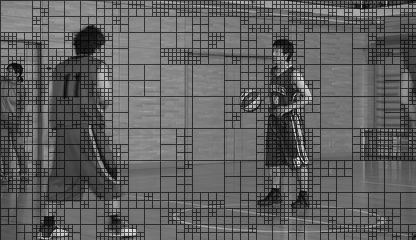
\includegraphics[width=0.5\linewidth]{./figures/partitioning-orig-all-001.png}}
	\\
	\subfloat[Predicted Image]
	{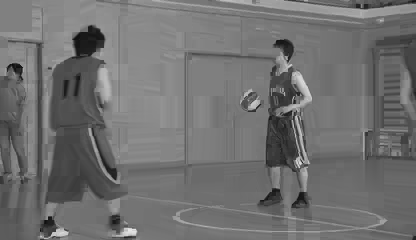
\includegraphics[width=0.5\linewidth]{./figures/pred_image-all-001.png}}
	\\
	\subfloat[Residual Image]
	{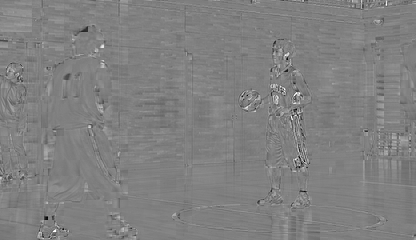
\includegraphics[width=0.5\linewidth]{./figures/res_image-all-001.png}}
	\caption{Example of an image at different encoding points for a
	certain level of quantisation}
	\label{fig:part_orig_pred_res_image}
\end{figure}

\subsubsection{Intra prediction}
\label{ssub:intra_prediction}
\index{intra prediction}

Intra prediction, sometimes referred to spatial prediction, is used to
eliminate spatial redundancies by removing the correlation with local regions
of a picture.
The basic principle of intra prediction is based on the fact that the texture
of a picture region is similar to the texture of its neighbourhood and can be
predicted from there.
Images coded using this technique exclusively are named I-frames.

Different models of predictions can be used through projections of adjacent
decoded blocks.
These models include directional projections, gradient projections (called
planar) and the projection of the mean value (called DC).
These \acp{IPM} are used to derive the predictions of the current block from
its the available boundaries, formed by reconstructed blocks.
The top-right part of figure~\ref{fig:mdcs} presents the average
\ac{HEVC} $4\times4$ residuals by scanning mode, together with their
representation in the transform domain.
The average residual profiles have lower (dark) values near the
available borders, which increase with the distance from the
boundaries: residuals issued from horizontal and vertical \acp{IPM} only
have the left and upper borders available, respectively, whereas the
remaining \acp{IPM} tend to have both borders available.
It can also be observed that the scanning patterns match reasonably well
the transform coefficients in each case, sorting them in an increasing
order.

With regards to previous standards, such as H.264/\ac{MPEG}-4 \ac{AVC}, which
has 9 different prediction modes for intra coding, \ac{HEVC} has an improved
prediction system, with 35 different prediction modes.
The upper-left part of figure~\ref{fig:mdcs} illustrates them.
A detailed explanation on how predictions are derived from the block
boundaries using those prediction modes can be found in Chapter 6 from Wien's
book on \ac{HEVC}~\cite{wien-15-hevc}.

\begin{figure}[tb]
	\centering
	\begin{minipage}{0.48\textwidth}
		\includegraphics{./figures/pred-directions.pdf}
	\end{minipage}
	\begin{minipage}{0.48\textwidth}
		\centering
		\small
		Average profile for residuals (prediction direction)
		\begin{tabular}[H]{ccc}
			
\includegraphics[width=0.25\textwidth]{figures/resids-scan-diag.png}
			&
			
\includegraphics[width=0.25\textwidth]{figures/resids-scan-horz.png}
			&
			
\includegraphics[width=0.25\textwidth]{figures/resids-scan-vert.png}
			\\
			\color{red}{diagonal} & \color{greenish}{vertical} & \color{blue}{horizontal} \\
			& & \\
		\end{tabular}
		\\
		\small
		Average profile for coefficients (scanning mode)
		\begin{tabular}[H]{ccc}
			
\includegraphics[width=0.25\textwidth]{figures/coeffs-scan-diag.png}
			&
			
\includegraphics[width=0.25\textwidth]{figures/coeffs-scan-horz.png}
			&
			
\includegraphics[width=0.25\textwidth]{figures/coeffs-scan-vert.png}
			\\
			\color{red}{diagonal} & \color{greenish}{horizontal} & \color{blue}{vertical} \\
		\end{tabular}
	\end{minipage}
	\subfloat[Diagonal scanning]{\includegraphics{figures/mdcs-diag.pdf}}
	\subfloat[Horizontal scanning]{\includegraphics{figures/mdcs-horz.pdf}}
	\subfloat[Vertical scanning]{\includegraphics{figures/mdcs-vert.pdf}}
	\caption{\acs{HEVC} intra prediction modes related to their average
	residual signals and their appropriate scanning in the transform
	domain for $4\times4$ \acsp{TU}}
	\label{fig:mdcs}
\end{figure}


\subsubsection{Inter prediction}
\label{ssub:inter_prediction}
\index{inter prediction}

Inter prediction, or temporal prediction, takes advantage of the fact that
images close in time share many similarities, and that some of their component
regions will move as a whole.
Since the encoding order is not necessarily the same as the viewing one, inter
predictions can have their origins in either past or future frames, and also
combine the two origins.
Images that are predicted using only one image either from the past or from
the future are called predicted images or P-frames.
Bi-predicted images or B-frames have prediction origins in two different
images.

At the encoder side, an extra operation, called motion estimation, is
carried out.
This stage searches for the best matching area in the reference picture
for the current prediction block.
It is one of the most complex parts of video coders in terms of computational
requirements.
Once a good prediction has been found, a motion vector is created, indicating
the offset that has to be applied in the block from the reference image.

\subsection{Transform}
\label{sub:transform}

The transform stage reduces the remaining correlations from the residual
block, computed as the difference between the original and the predicted
blocks.
The goal of the transform is to concentrate the residual signal into as few
coefficients as possible in the transform domain.
The residual signal is transformed from the spatial domain into the
transformed one using the transform.
In the spatial domain, the residual signal is spread among the pixels of the
blocks, while the objective of transform domains is to concentrate as much as
possible the residual signal into a few transform domain coefficients
exhibiting a large amplitude and the rest might be considered negligible.

This idea of the energy compaction is the main property of the transform
stage.

Most of the transforms used in standardised video coding schemes belong to the
\ac{DTT} family.
Amongst those, the \ac{DCT} of type II has received a considerable amount of
attention in the past and is the \emph{de facto} standard transform used in
\acs{ITU} and \acs{MPEG} codecs since \acs{MPEG}-1/H.261.

Additional choices were introduced recently, especially in \ac{HEVC}, where
the \ac{DST} of type VII was adopted.

The average profiles for some $4\times4$ intra residuals in \ac{HEVC} are
displayed in the upper-right part of figure~\ref{fig:mdcs}, along with their
corresponding representations in the transform domain.

Provided that the subject of this thesis is centred around the
transforms for video coding, the transform stage will be explained
thoroughly in Chapter~\ref{cha:transform_coding}.

\subsection{Quantisation}
\label{sub:quantisation}
\index{QP}\index{lossy}\index{lossless}

The quantisation, applied in the transform domain, it is used as an
approximation operator, reducing the amount of possible output values.
In standards like \ac{HEVC}, the quantisation is scalar:
each coefficient is approximated independently from its neighbouring values.
In these coding schemes, the quantisation step is controlled by a \ac{QP} that
discards any coefficient whose energy level is below a certain threshold.
High energy coefficients are also be affected by the quantisation.
In standards like \acs{HEVC}, the quantisation step is controlled by a
\ac{QP} that regulates the amount of approximations carried out.
It is worth noticing that it is the only non-reversible step in the whole
hybrid video coding scheme, which induces lossy video coding.
Lossless (or near-lossless) video coding can be attained by not using
quantification in the process.

\subsection{Entropy coding}
\label{sub:entropy_coding}
\index{CABAC}

The last operation consists in reducing the amount of bits transmitted through
the use of an entropy code.
This is a lossless operation, as such the bit reduction performed during this
stage is completely reversible: no approximation operation is performed at
this stage.

Once the transform coefficients have been quantised, they are processed to
conform the bitstream.
That is, the transform coefficients are scanned to make sure they are
sorted in a way that will make the entropy coder work more efficiently.

The scanning operation is a conversion from a 2D array, containing the
quantised transformed coefficients, towards 1D vector containing the same
values sorted in a way that facilitates a compact transmission.
For instance, in \ac{HEVC}, depending on the selected \ac{IPM}, residuals
present different patterns, and so do their transforms, as illustrated in
figure~\ref{fig:mdcs}.
These patterns in the transform domain will determine different scanning
orders (in different colours), as presented in the lower part of
figure~\ref{fig:mdcs}.
An adapted mode to different patterns ensures, in average, a correct order of
the coefficients that will group all the zeroes
together.
The patterns are described for $4\times4$ blocks, and the same pattern is used
on higher block sizes, which are recursively split into 4 sub-blocks until
size $4\times4$ is reached~\cite{sole-12-transform-coefficient-coding}.
An appropriate scanning is crucial for the entropy
coding~\cite{ye-08-intra-directional-scanning-mddt}.

Signalling is also conveyed into the bitstream at this point, and the
entropy coder ensures a correct binarisation while using the adequate
number of bits thanks to the \ac{CABAC}.

\section{Encoder control}
\label{sec:encoder_control}

The encoder control is used by essentially all blocks in the diagram
from figure~\ref{fig:hybrid_video_coding_scheme}.
This set of operations allow the encoder to take decisions related to coding
based on the application requirements.
These decisions include the block sizes and the prediction to use.
For each block size and kind of prediction, the encoder computes the
distortion, using its own decoder, and estimates the rate as illustrated in
figure~\ref{fig:rate_distortion_scheme}.

The appropriate set of choices, mainly among the prediction modes and block
sizes, is performed by comparing the Lagrangian values, which balance the
distortion and rates obtained for each coding choice.

Depending on the coding configuration, the encoder may also decide whether to
use references from the current image or from other images.
The \ac{AI} configuration, encodes each image independently from the rest,
whereas in the \ac{RA} configuration, the images conforming the sequences are
organised into \acp{GOP}, formed by an I-frame, and several P and B-frames.

\begin{figure}[tb]
	\centering
	\includegraphics{./figures/rate_distortion_scheme.pdf}
	\caption{Rate-distortion scheme of a transform-based codec}
	\label{fig:rate_distortion_scheme}
\end{figure}

\subsection{Distortion measures}
\label{sub:distortion_measures}

\subsubsection{Mean squared error}
\label{ssub:mean_squared_error}
\index{MSE}

The \ac{MSE} is the average of the square difference between two
signals.
For two-dimensional signals, such as images, the \ac{MSE} can be computed as:

\begin{equation}
	MSE_{I,K} = \frac{1}{m\,n} \sum\limits_{i=0}^{m-1} \sum\limits_{j=0}^{n-1}
	{\left[ I(i,j) - K(i,j) \right]} ^2
	\label{eqn:mse}
\end{equation}

Where $I$ and $K$ are two images of $m \times n$ pixels.

\subsubsection{Peak signal-to-noise ratio}
\label{ssub:peak_signal_to_noise_ratio}
\index{PSNR}

The \ac{PSNR} is also an objective measure of quality that computes the ratio
between the maximum possible value of a signal and the power of the noise that
affects the fidelity of its approximation.
It is usually defined in terms of the logarithmic decibel scale to cope
with the wide range that signals might have.
Defining the \ac{PSNR} in terms of the \ac{MSE} from
\eqref{eqn:mse}, it can be expressed as:
\begin{equation}
	PSNR = 10 \log_{10} \left(\frac{MAX_I^2}{MSE_{I,K}}\right)
	= 20 \log_{10} (MAX_I) - 10 \log_{10} (MSE_{I,K})
	\label{eqn:psnr}
\end{equation}
For 8-bit depth images, which are the main format considered in this thesis,
the maximum pixel values writes: $MAX = 2^{8} - 1 = 255$.

\subsection{Rate-distortion optimisation}
\label{sub:rate_distortion_optimisation}
\index{RDO}

In order to carry out the most sensible decision at each time, the
encoder uses a \ac{RDO} criterion
\cite{sullivan-98-rdo-video-compression}.

Each time the encoder has to make a decision about choosing a
particular block size for the partitioning or a prediction mode, it
checks the distortion that decision might cause as well as an estimation
of the bit rate needed.
The encoder performs this computation iteratively the same block,
exploring many different coding possibilities and finally selects the
one that provides the best score in terms of rate and distortion.
This is called the \ac{RDO} loop.
For instance, in \ac{HEVC}, it allows choosing the best \ac{PU} size
(4,8,16,32,64), \ac{TU} size (4,8,16,32), \ac{IPM} (0,1,\ldots,34), prediction
source (intra, inter), amongst others.

The trade-off between the distortion and the rate is commonly expressed
using a Lagrangian measure.

\begin{equation}
	J(\lambda) = \text{Distortion} + \lambda \text{Rate}
	\label{eqn:lagrangian_rdo}
\end{equation}

As seen in the previous subsections, computing the distortion is
reasonably straightforward.
However, estimating the bit rate is a bit more delicate, since the whole
entropy coder cannot be run each time the encoder explores the different
possibilities for a block.
As a consequence, an estimation of the bit rate is often used in the \ac{RDO}
loop.

Next chapter will present a way of using~\eqref{eqn:lagrangian_rdo} to design
performing transforms based on different rate models.

\section{Bj{\o}ntegaard Delta measurements}
\label{sub:bjontegaard_delta_measurements}
\index{BD-rate}
\index{BD-PSNR}

Comparing two video coding techniques objectively might be complicated,
as both distortion and bit rate savings have to be taken into account jointly.

Metrics introduced by Gisle Bjøntegaard, know as \ac{BD} measurements have
become the current \emph{de facto} standard to objectively compare the result
of two encodings~\cite{VCEG-M33,VCEG-AI11}.
Two different metrics are defined and displayed in
figure~\ref{fig:bdsnr_bdrate}:
\begin{enumerate}[label = (\alph{enumi})]
	\item \ac{BD}-\ac{PSNR}: computes the relative quality improvement
		in \deci\bel.
	\item \ac{BD}-rate: computes the relative savings in bit rate for an
		equivalent distortion in percent.
\end{enumerate}

\begin{figure}[tb]
	\centering
	\subfloat[\acs{BD}-\acs{PSNR}]
	{\includegraphics{./figures/bd_psnr_plot.pdf}}
	\hfill
	\subfloat[\acs{BD}-rate]
	{\includegraphics{./figures/bd_rate_plot.pdf}}
	\caption{Schematic representation of rate-distortion plots using the
	\acs{BD} measurements}
	\label{fig:bdsnr_bdrate}
\end{figure}

The \ac{BD}-rate measurement will be used extensively in this thesis to
appreciate the performance of the proposed systems.

\section{Conclusions}
\label{sec:conclusions_video_coding}

This chapter has presented the motivation for video coding as well as some
general concepts concerning an overview of the video coding system.

Current video coders exploit redundancies existing within images of the video
sequence via predictions.
These predictions can be either spatial or temporal, depending on
whether the prediction source is the same image or another image,
respectively.
Unpredictable parts of the image, called residuals, are then passed through a
transformation in order to concentrate the transformed residual in as few
coefficients as possible.

The appropriate block size is selected for the prediction and the transform
sizes, named \acp{PU} and \acp{TU}, respectively.
A lot of flexibility is allowed in the syntax for the prediction and sizes
while the set of choices for a given codec is rather limited for the
transform.

This thesis will focus on the extension of the choices for the transform
stage.
Currently, the decision of the coding mode (\ac{AI}, \ac{RA}), the block sizes
and \acp{IPM} are is based on a single transform, usually the \ac{DCT}-II.
However, a single transform cannot provide optimal signal compaction for all
kinds of possible signals.

This thesis will focus on the extension of the choices for the transform
stage, as set of transforms will be provided such that the encoder is able to
better adapt the transform to the varying nature of the prediction residuals.

Next chapter will explore the details of the transforms used in video coding,
namely their design principles and a comparison between two design approaches.

\chapter{Transform coding}
\label{cha:transform_coding}
\chaptertoc

\section{Introduction to transforms}
\label{sec:introduction_to_transforms}

In the previous chapter, transforms were mentioned as an important part
in current video coders.
This chapter will study their design and properties that lead transforms
to be useful in video coding.

A transform is a mathematical operation that takes an input signal and
represents the same input signal in a different domain.

High energy compaction provided by transform coding has led this
technique to be present in all the international video coding standards.

Transform coding allows reducing existing signal correlations in the
spatial domain, leading to a more decorrelated signal in the transform
domain and ensuring a more compact representation.
This is of great importance for the upcoming stages of scanning and
entropy coding.

Transforms can be very abstract since they tend to work in $N$-dimensional
spaces, where $N$ represents the number of pixel residuals processed by the
transform.
Typical values vary from $N=4\times4$ to $N=32\times32$ using powers of two in
modern video codecs, such as \ac{HEVC}.

However, restraining ourselves to two dimensions, one of the most visual
and representative example of transforms are rotations.
The example in figure~\ref{fig:transform_rotation} helps visualising the
transform role in signal compression.

\begin{figure}[tb]
	\centering
	\includegraphics{./figures/transform_rotation_plot.pdf}
	\caption{Simple transform performing a rotation}
	\label{fig:transform_rotation}
\end{figure}

Whereas on the left signal (in blue), both coordinates are needed to describe
the signal accurately, on the right signal (in red), one coordinate, namely
the vertical dimension is enough to provide an equally accurate signal
representation, since the horizontal dimension remains constant.

\subsection{Block transforms}
\label{sub:block_transforms}

Block-based coding is widely adopted in image/video systems, such as
\acs{JPEG}, \ac{AVC} and \ac{HEVC}.
In these systems, an image is divided into non-overlapping blocks and for each

In these systems, the image to be transformed is split into non-overlapping
blocks, and each one will be transformed independently.
Although this has the disadvantage of not being able to exploit correlations
of different blocks, contrary to wavelet transforms used in \acs{JPEG}
2000~\cite{jpeg2000}, the block-based scheme leads to a reduced complexity and
allows treating each block differently according to its
content~\cite{xu-09-intra-predictive-transforms}.

Since block transforms are used exclusively in state-of-the-art video coding
systems, they will be the targeted type of transforms in this thesis.

\subsection{Orthogonal transforms}
\label{sub:orthogonal_transforms}

Transforms used in image processing and video coding are orthogonal.
Orthogonal matrices are square matrices whose rows and columns are orthogonal
unit vectors, also known as orthonormal vectors, with:
\begin{equation}
	\A^T\A = \A\A^T = \I
\end{equation}
As a consequence, the inverse matrix of an orthogonal matrix is its
transposed version:
\begin{equation}
	\A^T = \A^{-1}
\end{equation}

This property has benefits in two areas: fast computation of inverse transform
with no need to store it separately and re-use of fast algorithms for both
direct and inverse transform applications.

\subsection{Separability}
\label{sub:separability}

Image and video coding deal with image blocks, which are two-dimensional
signals and, consequently, use transforms able two process those
signals.

The naive approach to work with those signals is to use non-separable
transforms.
These transforms take the residual pixels from a block and reshape it to a
single-dimensional signal. For instance, a $4\times4$ block of pixels becomes a
$16\times1$ vector.
Afterwards the transform is applied normally:
\begin{equation}
	\X = \A \, \x
\end{equation}
where $\x$ is a $N \times N$ block, reshaped into a $N^2\times1$ vector
and $\A$ is a $N^2 \times N^2$ matrix.
The main disadvantage of this approach is the number of calculations
required to obtain the transformed signal: for a $N \times N$ block, the
number of operations required to transform it in a non-separable way is:
$N^4$ multiplications and $N^2(N^2-1)$ additions.

\begin{figure}[tb]
	\centering
	\includegraphics{./figures/block_linearisation.pdf}
	\caption{Example of a $4\times4$ block linearisation}
	\label{fig:block_linearisation}
\end{figure}

On the other hand, any linear correlation can be exploited between any pixel
within a block:
complex relationships between distant pixels can be handled regardless their
position in the block.

Due to the high amount of operations needed to transform a block, using
non-separable transforms, separable transforms are widely used in video
coding.
A block is transformed using horizontal and vertical separable transforms
$\A_h, \A_v$ for rows and columns, respectively, as:
\begin{equation}
	\X = \A_v {\left(\A_h \, \x^T\right)}^T = \A_v \, \x \, \A_h^T
	\label{eqn:sep_transform}
\end{equation}
The operation inside the parenthesis transforms the rows of $\x$, and
the outer part, the columns of $\x$.
By performing the horizontal and vertical transforms separately, the
number of operations required has been reduced to $2N^3$ multiplications
and $2N^2(N-1)$ additions.

However, this reduction in complexity comes at a price: non-separable
transforms were able to exploit any correlation amongst pixels within a
block, whether separable transforms can only decorrelate pixels that
share the same row or column.
In other words, separable transforms might be less performing than their
non-separable counterparts.
The impact in performance due to separability will be studied in detail
in Chapter~\ref{cha:the_mode_dependent_directional_transforms}.

A non-separable transform can be expressed from a set of two separable
transforms via the Kronecker product, denoted as $\otimes$.
\begin{equation}
	\mathbf{A}\otimes\mathbf{B} = 
	\begin{bmatrix}
		a_{11} \mathbf{B} & \cdots & a_{1n}\mathbf{B} \\
		\vdots & \ddots & \vdots \\
		a_{m1} \mathbf{B} & \cdots & a_{mn} \mathbf{B}
	\end{bmatrix}
\end{equation}
Where $\mathbf{A}$ is an $m \times n$ matrix and $\mathbf{B}$ is a $p \times
q$ matrix.
More explicitly:
\begin{equation}
	\mathbf{A}\otimes\mathbf{B} =
	\begin{bmatrix}
		a_{11} b_{11} & a_{11} b_{12} & \cdots & a_{11} b_{1q} & \cdots & \cdots & a_{1n} b_{11} & a_{1n} b_{12} & \cdots & a_{1n} b_{1q} \\
		a_{11} b_{21} & a_{11} b_{22} & \cdots & a_{11} b_{2q} & \cdots & \cdots & a_{1n} b_{21} & a_{1n} b_{22} & \cdots & a_{1n} b_{2q} \\
		\vdots & \vdots & \ddots & \vdots & & & \vdots & \vdots & \ddots & \vdots \\
		a_{11} b_{p1} & a_{11} b_{p2} & \cdots & a_{11} b_{pq} & \cdots & \cdots & a_{1n} b_{p1} & a_{1n} b_{p2} & \cdots & a_{1n} b_{pq} \\
		\vdots & \vdots & & \vdots & \ddots & & \vdots & \vdots & & \vdots \\
		\vdots & \vdots & & \vdots & & \ddots & \vdots & \vdots & & \vdots \\
		a_{m1} b_{11} & a_{m1} b_{12} & \cdots & a_{m1} b_{1q} & \cdots & \cdots & a_{mn} b_{11} & a_{mn} b_{12} & \cdots & a_{mn} b_{1q} \\
		a_{m1} b_{21} & a_{m1} b_{22} & \cdots & a_{m1} b_{2q} & \cdots & \cdots & a_{mn} b_{21} & a_{mn} b_{22} & \cdots & a_{mn} b_{2q} \\
		\vdots & \vdots & \ddots & \vdots & & & \vdots & \vdots & \ddots & \vdots \\
		a_{m1} b_{p1} & a_{m1} b_{p2} & \cdots & a_{m1} b_{pq} & \cdots & \cdots & a_{mn} b_{p1} & a_{mn} b_{p2} & \cdots & a_{mn} b_{pq} 
	\end{bmatrix}
\end{equation}

\subsection{Transform design}
\label{sub:transform_design}

Since the objective of the transforms is to be able to represent the signal
with as few coefficients as possible while minimising the distortion
introduced by the quantisation, transform design methods need to consider
trade-offs between the distortion and the number of bits needed to represent
those signals in the transform domain, as shown previously in
\S\ref{sub:rate_distortion_optimisation}.

Transform design methods agree on how the distortion is evaluated, namely
using the \ac{MSE} from~\eqref{eqn:mse}.
However, different transform designs exist depending on how the bit-rate is
estimated and modelled.

Next sections will study different transform design approaches based on
different modellings of the rate constraint.
\section{The Karhunen-Loève transform}
\label{sec:the_karhunen_loeve_transform}
\index{KLT}
The components of source signals within a residual block are correlated with
one another.
This correlation is expressed in terms of a correlation matrix containing the
linear inter pixel correlations.
For two $N$-dimensional signals $\x,\y$, the covariance signal between them
can be computed as:
\begin{align}
	\nonumber
	\C_{\x,\y} & = \E\left\{\x\y^T\right\} =
	\E\left\{
	\begin{bmatrix}
		x_0 \\ x_1 \\ \vdots \\ x_{N-1}
	\end{bmatrix}
	\begin{bmatrix}
		y_0 & y_1 & \cdots & y_{N-1}
	\end{bmatrix}
	\right\} \\
	& = \E\left\{
	\begin{bmatrix}
		x_0y_0 & x_0y_1 & \hdots & x_{0}y_{N-1} \\
		x_1y_0 & x_1y_1 & \hdots & x_{1}y_{N-1} \\
		\vdots & \vdots & \ddots & \vdots \\
		x_{N-1}y_0 & x_{N-1}y_1 & \hdots & x_{N-1}y_{N-1}
	\end{bmatrix}
	\right\} \\ \nonumber
	& =
	\begin{bmatrix}
		\E\left\{x_0y_0\right\} & \E\left\{x_0y_1\right\} & \hdots & \E\left\{x_{0}y_{N-1}\right\} \\
		\E\left\{x_1y_0\right\} & \E\left\{x_1y_1\right\} & \hdots & \E\left\{x_{1}y_{N-1}\right\} \\
		\vdots & \vdots & \ddots & \vdots \\
		\E\left\{x_{N-1}y_0\right\} & \E\left\{x_{N-1}y_1\right\} & \hdots & \E\left\{x_{N-1}y_{N-1}\right\}
	\end{bmatrix}
\end{align}
If $\x=\y$, the covariance matrix is the correlation matrix of $\x$.

It is possible to select an orthogonal matrix $\A$, for a given \ac{PDF}
describing the source that will make $\X=\A\x$ have pairwise uncorrelated
components in the transform domain~\cite{gersho-92-vector-quantization}.
The \ac{KLT} is defined as the linear orthogonal transform that reduces the
redundancy by a maximum decorrelation of the data, so that the signal can be
stored more efficiency~\cite{rao-01-transform-data-compression-book}.

In this section, the \ac{KLT} is presented under its well-known optimal
conditions: Gaussian sources with high resolution quantisation
assumptions~\cite{goyal-00-high-resolution}.
The high resolution assumption states that the number of quantisation levels
is high and the quantisation step size is small enough to consider the
\ac{PDF} constant for each quantisation interval.

Under those conditions, the \ac{KLT} is the transform that achieves optimal
bit allocation for the quantisation of transform coefficients by distributing
their variances in such a way as to minimise their geometric
mean~\cite{jayant-84-digital-coding-waveforms}, while minimising the overall
distortion~\cite{gersho-92-vector-quantization}.

The \ac{KLT} decorrelates the signal in the transform domain, that is the
correlation function of the signal in the transform domain $\C_\X$ is a
diagonal matrix, which can be computed as follows.
Let $\x$ be a zero-mean process and $\A$ an orthogonal transform, then, in
the transform domain:
\begin{equation}
	\X = \A \x \qquad \text{s.t. } \A \A^T = \I
\end{equation}
The covariance matrix in the transform domain is expressed as:
\begin{equation}
	\C_\X = \E\left\{\X \X^T\right\} = \A \E\left\{\x\x^T\right\}\A^T =
	\A\C_\x\A^T
\end{equation}
Or equivalently:
\begin{equation}
	\A^T\C_\X = \C_\x\A^T
\end{equation}
And since $\C_\X$ is diagonal:
\begin{equation}
	\C_\x \a_i = \lambda_i\a_i
\end{equation}
Where:
\begin{itemize}
	\item $\a_i$ are the eigenvectors of $\C_\x$.
	\item $\lambda_i$ are the eigenvalues of $\C_\x$.
\end{itemize}

\subsection{Particular case on natural images: the \acs{DCT}}
\label{sub:particular_case_dct}
\index{DCT}
\index{Markov}
\index{AR}
\index{Toeplitz matrix}

One of the most used transforms in image and video coding is the
\acf{DCT}.
In this section, the \ac{DCT} is justified over a particular kind
of signals: natural images.
The statistics of pixels in natural images match closely a first order
\ac{AR} process.
A first order \ac{AR} model, also known as Markov-1 process, is a stochastic
process that can be generated through the following regression formula:
\begin{equation}
	x(n) = \rho x(n-1) + w(n)
	\label{eqn:first_order_ar_model}
\end{equation}
Where $\rho$ is the correlation coefficient between two adjacent samples
and $w(n)$ is a white noise with zero mean, whose variance is related to
the variance of $x(n)$ $\sigma_x^2$ as:
\begin{equation}
	\sigma_w^2 = \E\left\{ w(n) w(n) \right\} =
	\left(1-\rho^2\right)\sigma_x^2
\end{equation}
The correlation matrix of this process takes the form of a Toeplitz
matrix~\cite{akansu-12-toeplitz-approximation}:
\begin{equation}
	\R_x = \sigma_x^2
	\begin{pmatrix}
		1          & \rho       & \rho^2     & \cdots & \rho^{N-1} \\
		\rho       & 1          & \rho       & \cdots & \rho^{N-2} \\
		\rho^2     & \rho       & 1          & \cdots & \rho^{N-3} \\
		\vdots     & \vdots     & \vdots     & \ddots & \vdots     \\
		\rho^{N-1} & \rho^{N-2} & \rho^{N-3} & \cdots & 1
	\end{pmatrix}
	\label{eqn:toeplitz_matrix}
\end{equation}
The \ac{KLT} for this kind of processes, that is, the eigenvectors of
$\R_\x$, tends to the \ac{DCT} as $\rho\to1$~\cite{britanak-06-dct-and-dst}.
The \ac{DCT}-II can be expressed compactly as:
\begin{equation}
	{\left[C_{N}^{II} \right]}_{n,k} =
	\sqrt{\frac{2}{N}}\epsilon_k\cos\left(\frac{\pi(2n+1)k}{2N}\right)
	\quad
	n,k=0,\dots,N-1
	\label{eqn:dct_ii}
\end{equation}

\begin{equation}
	\epsilon_k =
	\begin{cases}
		\frac{1}{\sqrt{2}} & k = 0 \\
		1 & \text{otherwise}
	\end{cases}
\end{equation}

The fact that the \ac{DCT} approximates the \ac{KLT} for image signals and its
efficient implementation has made it the preferred choice in image and video
compression algorithms to decorrelate the signals and provide optimal bit
allocation~\cite{sole-12-transform-coefficient-coding}.

\begin{figure}[tb]
	\centering
	\subfloat[\acs{DCT}-II $4\times4$]
	{
\includegraphics[width=0.3\linewidth]{./figures/dct4-bases.png}}
	\hspace{0.2\linewidth}
	\subfloat[\acs{DST}-VII $4\times4$]
	{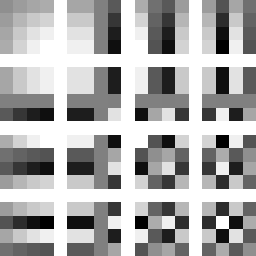
\includegraphics[width=0.3\linewidth]{./figures/dst4-bases.png}}
	\caption{Transforms used in \acs{HEVC} for $4\times4$ blocks}
	\label{fig:dct_dst}
\end{figure}

\subsection{Particular case on prediction residuals: the \acs{DST}}
\label{sub:particular_case_dst}
\index{DST}
\index{intra prediction}
\index{tridiagonal matrix}
\index{Toeplitz matrix}

Although the \ac{DCT} has been proved to be nearly the \ac{KLT} for natural
images, it is used in predictive transform coding based video standards.
This kind of coding leads to signals whose nature differs from that of
natural images: prediction residuals.
In particular, prediction residuals resulting from intra prediction tend
to have particular properties.
Those residuals are computed using predictions from already
reconstructed blocks, usually available on the left and upper borders (in
grey) of the current residual (in white), as shown in
figure~\ref{fig:pred_scheme}.a.
An example of an average intra prediction residual is provided in
figure~\ref{fig:pred_scheme}.b.
It can be noticed that the energy of the residual is lower (dark) near
the borders where reconstructed blocks are available, and that the error
gets higher (lighter) as one moves away from the boundaries.
These properties motivated a study on this particular kind of blocks,
resulting in a transform that performs better on them than the \ac{DCT}:
the \acf{DST}~\cite{han-10-spatial-adaptive-transform}.
\begin{figure}[tb]
	\centering
	\subfloat[Intra prediction modes for the current block (white) from
	previously reconstructed blocks (grey)]
	{\includegraphics{./figures/pred-scheme.pdf}}
	\hspace{0.2\linewidth}
	\subfloat[Average intra prediction residual]
	{
\includegraphics[width=0.3\linewidth]{./figures/resids-scan-diag.png}}
	\caption{Prediction scheme showing all intra prediction modes and a
	prediction residual example}
	\label{fig:pred_scheme}
\end{figure}

Intra prediction residuals present a correlation matrix that can be modelled
using a Toeplitz tridiagonal matrix, as the one
in~\eqref{eqn:tridiagonal_matrix}~\cite{han-10-spatial-adaptive-transform,
yueh-05-eigenvalues-tridiagonal}.
Those eigenvalues can be expressed in a closed form using the \ac{DST}-VII
from~\eqref{eqn:dst_vii}.

\begin{equation}
	\tilde\R_x =
	\begin{pmatrix}
		1+\rho^2 & -\rho    & 0        & 0      & \hdots & 0            \\
		-\rho    & 1+\rho^2 & -\rho    & 0      & \hdots & 0            \\
		0        & -\rho    & 1+\rho^2 & -\rho  & \hdots & 0            \\
		0        & \ddots   & \ddots   & \ddots & \ddots & \vdots       \\
		\vdots   & \ddots   & \ddots   & \ddots & \ddots & -\rho        \\
		0        & \hdots   & 0        & 0      & -\rho  & 1+\rho^2-\rho
	\end{pmatrix}
	\label{eqn:tridiagonal_matrix}
\end{equation}

\begin{equation}
	{\left[S_{N}^{VII} \right]}_{n,k} =
	\frac{2}{\sqrt{2N+1}}\sin\left(\frac{\pi(2n-1)k}{2N+1}\right),
	\quad
	n,k = 1, \dots, N
	\label{eqn:dst_vii}
\end{equation}

Figure~\ref{fig:dct_dst}.b presents the \ac{DST}-VII bases for
$4\times4$ blocks.
The resemblance between an average residual block from
figure~\ref{fig:pred_scheme}.b can be spotted by comparing it to the first
base vector from the \ac{DST}.

The use of the \ac{DST} in \ac{HEVC} over the \ac{DCT} on $4\times4$
blocks leads to a bit-rate reduction of 1\% on
average~\cite{sullivan-12-overview-hevc}.

An explanation on the adoption of the \ac{DST} into \ac{HEVC} is detailed in
Chapter~\ref{cha:the_mode_dependent_directional_transforms}, more precisely in
\S\ref{sub:dst_and_mddt}.

\subsection{Final note on the \acs{KLT}}
\label{sub:final_note_on_the_klt}

The \ac{KLT} is often presented as the optimal transform, sometimes even for
all possible sources of signals.
However, it has been proved to be suboptimal in the transform coding / bit
allocation sense in some cases~\cite{effros-04-suboptimal-klt}.
For this reason, next section studies another kind of transform design that
leads to optimal transforms under different conditions.

\section{The rate-distortion optimised transform}
\label{sec:the_rate_distortion_optimised_transform}
\index{RDOT}

As discussed before, transforms try to find a compact representation of the
signal in the transform domain.
The \ac{KLT}, under certain assumptions, provides optimal bit allocation and
signal decorrelation.

Sezer proposes an alternative kind of transforms to minimise the trade-off
between the distortion and the rate from~\eqref{eqn:lagrangian_rdo} by taking
into account the sparsity of the output signal in their
design~\cite{sezer-11-phd,sezer-08-sparse-orthonormal-transforms}.
This transform, named \ac{RDOT}, contrary to the \ac{KLT}, does not make use
of the high resolution assumption.
Instead, the bit-rate constraint is modelled via the sparsity of the
transformed coefficients, by the introduction of the $\ell_0$ norm, which
counts the number of non-zero coefficients in a vector.
The proposed \ac{RDOT} can be expressed as:
\begin{equation}
	\A_{opt} = \arg\min\limits_{\A}
	\sum_{\forall i} \min\limits_{\c_i}
	\left(
	{\Vert \x_i - \A^T\c_i \Vert}_2^2 + \lambda{\Vert \c_i \Vert}_0
	\right)
	\label{eqn:rdot-nsep}
\end{equation}
Where $\x_i$ are the input signals, i.e.\ a block of the training set,
$\c_i$ are its quantised transformed coefficients using the transform
$\A$.
$\A^T$ is its transposed matrix, as $\A$ is chosen orthogonal.
The constraint in the cost function is the average $\ell_0$ norm of the
coefficients, i.e.\ the number of non-zero coefficients.
Finally, $\lambda$ is the Lagrange multiplier of the constraint.

The fact that this transform design strives to obtain sparse signals in the
transform domain fits the state-of-the-art video coding standard, \ac{HEVC}.
There are even syntax elements in \ac{HEVC} that deal with sparsity:
for a given transformed residual, the position of the last non-zero value is
signalled, meaning that, instead of explicitly transmitting all the following
zeroes, it is indicated that from that point onwards, all the following values
are zero.

A thorough study of~\eqref{eqn:rdot-nsep} analysing its properties and
consequences is detailed below.

\subsection{The \acs{RDOT} metric}
\label{sub:the_rdot_metric}

The value that \acp{RDOT} minimise is expressed
in~\eqref{eqn:rdot_metric} for a single signal.
This metric depends exclusively on the quantisation step $\Delta$ and the
initial transform used $\A$.
The relation between the Lagrange multiplier $\lambda$ and $\Delta$ is
detailed in \S\ref{sub:the_lagrange_multiplier}.
\begin{equation}
	J (\lambda) =
	{\Vert \x - \A^T \c \Vert}_2^2 + \lambda{\Vert \c \Vert}_0
	\label{eqn:rdot_metric}
\end{equation}
The first part of the equation represents the distortion introduced by
the quantisation.
The second term serves as rate-like constraint, by ensuring that the
number of significant values in the transform domain is minimised together
with the distortion.

The minimisation of the metric happens in two steps, carried out iteratively
until convergence:
\begin{enumerate}
	\item Finding the optimal coefficients for a given transform.
	\item Updating the transform for the optimal coefficients.
\end{enumerate}

\subsubsection{Optimal coefficients for a given transform}
\label{ssub:optimal_coefficients_for_a_given_transform}

The optimal coefficients that introduce the minimum distortion for a given
quantisation step $\Delta$ are obtained by transforming the signal and
hard-thresholing them:
\begin{equation}
	\c = \lfloor \X \rfloor = \lfloor \A \x \rfloor
\end{equation}
The threshold value is tightly related to the Lagrange multiplier $\lambda$,
as demonstrated in \S\ref{sub:the_lagrange_multiplier}:
\begin{equation}
	\c[n] =
	\begin{cases}
		\X[n] & \vert \X[n] \vert \ge \displaystyle \frac{\Delta}{2} \\
		0     & \text{otherwise} \\
	\end{cases}
	\label{eqn:hard_threshold}
\end{equation}

\subsubsection{Optimal transform for given coefficients}
\label{ssub:optimal_transform_for_given_coefficients}

Once the optimal coefficients have been found, the transform $\A$ must
be updated to provide the mapping between $\x$ and $\c$ while minimising
the reconstruction error.
\begin{equation}
	\A_{opt} = \arg\min\limits_{\A}
	\left(
	\sum_{\forall i}{\Vert \x_i - \A^T\c_i\Vert}^2
	\right)
	\qquad \text{s.t. } \A\A^T = \I
\end{equation}
Since the expression is a scalar value, it can be rewritten using the trace
(the sum of a matrix diagonal):
\begin{equation}
	\A_{opt} = \arg\min\limits_{\A}
	\left(\sum_{\forall i}\tr\left( 
	{\left(\x_i - \A^T\c_i\right)}^T\left( \x_i - \A^T\c_i\right)
	\right)\right)
\end{equation}
Operating:
\begin{equation}
	\A_{opt} = \arg\min\limits_{\A}
	\left(\sum_{\forall i}\tr\left( 
	\x_i^T\x_i -\x_i^T\A^T\c_i -\c_i^T\A\x_i + \c_i^T\A\A^T\c_i
	\right)\right)
\end{equation}
Since the trace is a linear operator and $\A\A^T=\I$:
\begin{equation}
	\A_{opt} = \arg\min\limits_{\A}
	\left(\sum_{\forall i}
	\tr\left(\x_i^T\x_i\right)
	-\tr\left(\x_i^T\A^T\c_i\right)
	-\tr\left(\c_i^T\A\x_i\right)
	+\tr\left(\c_i^T\c_i \right)
	\right)
\end{equation}
Making use of the cyclic property of the trace and removing
$\A$-independent terms:
\begin{equation}
	\A_{opt} = \arg\min\limits_{\A}
	\left(\sum_{\forall i}
	-2\tr\left(\c_i\x_i^T\A^T\right)
	\right)
\end{equation}
Defining $\Y=\displaystyle\sum_{\forall i}\c_i\x_i^T$ and its SVD
decomposition $\Y=\U\Lambdab^{\nicefrac{1}{2}}\V^T$, where $\U$ and $\V$
are orthogonal and $\Lambdab$ is a positive semi-definite diagonal matrix.
The equation rewrites as follows:
\begin{equation}
	\A_{opt} = \arg\min\limits_{\A}
	\left(
	-2\tr\left(\U\Lambdab^{\nicefrac{1}{2}}\V^T\A^T\right)
	\right)
\end{equation}
Minimising a negative expression is equivalent to maximise its positive
version.
Re-arranging the terms using the trace cyclic property:
\begin{equation}
	\A_{opt} = \arg\min\limits_{\A}
	\left(
	-2\tr\left(\Lambdab^{\nicefrac{1}{2}}\V^T\A^T\U\right)
	\right)
\end{equation}
Let $\Pb=\V^T\A^T\U$.
Since $\V$, $\A$ and $\U$ are orthogonal, so is $\Pb$.
The equation is now:
\begin{equation}
	\A_{opt} = \arg\max\limits_{\A}
	\left(
	\tr\left(\Lambdab^{\nicefrac{1}{2}}\Pb\right)
	\right)
\end{equation}
Since $\Lambdab$ is a diagonal matrix whose entries are non-negative by
definition and $\Pb$ is orthogonal, the maximisation is achieved when
$\Pb=\I$:
\begin{equation}
	\V^T\A_{opt}^T\U=\I\quad \Rightarrow \quad \A_{opt} = \U\V^T
\end{equation}

Summing up, the optimal transform is obtained using the SVD decomposition of
the covariance matrix between the output signal (the transformed and quantised
coefficients) with the input signal (the intra prediction residuals).

\subsection{Separable \acs{RDOT} design}
\label{sub:separable_rdot_design}

The methods for transform design and learning presented in the previous
sections are non-separable.
This means that the input block is linearised and then transformed in
one step.
Due to complexity issues, non-separable transforms are hardly used in
performing solutions.
A lower complexity approach involves separable transforms, which may not be
able to concentrate the energy in the transform domain as well as their
non-separable counterparts.
In order to design and learn separable transforms, the design and learning
methods have to be adapted.
In the case of the \ac{KLT} is straightforward to see that one can learn
a horizontal \ac{KLT} to transform the rows of the signal and a vertical
\ac{KLT} for the columns.
However, the \ac{RDOT} algorithm needs further tuning in order to obtain
separable transforms.
A possible way of learning a separable \ac{RDOT} was also proposed by
Sezer~\cite{sezer-11-phd} and validated by independent
researches~\cite{sole-09-sparsity-optimisation-separable-transforms}.
The proposed method consists in updating each one of the horizontal and
vertical transforms separately.

The separable transformation of a block $\x$ has been previously defined as a
two step transformation in~\eqref{eqn:sep_transform}:
\begin{equation*}
  \X = {\A_v\left( \A_h \x^T \right)}^T = \A_v \x \A_h^T
\end{equation*}

Where $\x$ is the two-dimensional block to transform, $\A_h$ is the horizontal
transform, used to transform the rows of $\x$ and $A_v$ is the vertical
transform, used to transform the columns of $\x$.

The equation to optimise using separable transforms reads as follows:
\begin{equation}
	\A_{v_{opt}}, \A_{h_{opt}} = \arg\min\limits_{\A_v,\A_h}
	\left(
	\sum_{\forall i} \min\limits_{\c_i}{\Vert \x_i - \A_v^T\c_i\A_h \Vert}_2^2
	+ {\Vert \c_i \Vert}_0
	\right)
	\label{eqn:rdot-sep}
\end{equation}

This minimisation problem can be solved in a similar way to the non-separable
version.

\subsubsection{Optimal coefficients for a given transform}
As in the non-separable problem, the optimal coefficients $\c_i$ are found by
hard-thresholding the components of $\X_i=\A_v\x_i\A_h^T$ with $\sqrt{\lambda}$.
\subsubsection{Optimal vertical transform for given coefficients}
Now, the vertical transform needs to be updated accordingly:
\begin{equation}
	\A_{v_{opt}} = \text{arg}\min\limits_{\A_v}
	\left(
	\sum_{\forall i} {\Vert \x_i - \A_v^T\c_i\A_h \Vert}_2^2
	\right)
	\qquad \text{s.t. } \A_v\A_v^T = \I
\end{equation}
Expanding the expression and grouping the terms as in the non-separable
the covariance matrix $\Y$ can be defined as:
\begin{equation}
\Y = \sum_{\forall i} \c_i\A_h\x_i =
\U\Lambdab^{1/2}\V^T
\end{equation}
Then the optimal transform is given by:
\begin{equation}
  \A_{v_{opt}} = \U\V^T
\end{equation}
\subsubsection{Optimal coefficients for updated vertical transform}
As in the non-separable problem, the optimal coefficients $\c_i$ are found by
hard-thresholding the components of $\X=\A_{v_{opt}}\x_i\A_h^T$ with
$\sqrt{\lambda}$. However, this time we use the optimal vertical transform from
the previous step.
\subsubsection{Optimal horizontal transform for given coefficients}
Now, the horizontal transform needs to be updated accordingly:
\begin{equation}
	\A_{h_{opt}} = \text{arg}\min\limits_{\A_h}
	\left(
	\sum_{\forall i} {\Vert \x_i - \A_{v_{opt}}^T\c_i\A_h \Vert}_2^2
	\right)
	\qquad \text{s.t. } \A_h\A_h^T = \I
\end{equation}
Expanding the expression and grouping the terms as in the non-separable
the covariance matrix $\Y$ can be defined as:
\begin{equation}
	\Y = \sum_{\forall i} \c_i^T\A_{v_{opt}}\x_i =
\U\Lambdab^{1/2}\V^T
\end{equation}
Then the optimal transform is given by:
\begin{equation}
	\A_{h_{opt}} = \U\V^T
\end{equation}

\subsection{The Lagrange multiplier and the zero norm}
\label{sub:the_lagrange_multiplier}
\index{generalised normal distribution}
\index{generalised Gaussian distribution}
\index{exponential power distribution}

Video coding residuals distribution can be modelled using a \ac{GGD}, also
known as generalised normal distribution or exponential power
distribution~\cite{lam-00-dct-coefficient-distribution,
yovanof-96-analysis-dct-coefficients}.
For this reason, in order to obtain the optimal Lagrange multiplier in a
reasonably general case, a \ac{GGD} will be used to represent the
residuals \ac{PDF}.

Figure~\ref{fig:probability_density_functions} illustrates the \acp{PDF}
of a set of residuals transformed with the \ac{DCT} and the same residuals
transformed with an adapted \ac{RDOT}.
As expected, the red curve, representing the \ac{RDOT} presents higher
sparsity than the generic \ac{DCT}:
its value is above the \ac{DCT} on zero, meaning that the resulting
coefficients have more zeros when using the \ac{RDOT}.
Using different the transforms, modifies the resulting \ac{PDF}, but since the
used transforms are orthogonal, the variance remains unaltered.
Residuals are computed as the difference between predicted and original
blocks, meaning they are prediction errors.
These errors are made by excess or defect evenly, evidenced by their
zero-mean \ac{PDF}.
\begin{figure}[tb]
	\centering
	\includegraphics{./figures/pdfs_plot.pdf}
	\caption{\acsp{PDF} of the residuals with different transforms
	compared to Laplace and normal distributions}
	\label{fig:probability_density_functions}
\end{figure}
Figure~\ref{fig:probability_density_functions} also includes the
\ac{PDF} of a Laplace distribution and a normal distribution.
Those two distributions are particular cases of a \ac{GGD}.

The centred \ac{GGD} \ac{PDF} can be expressed compactly as:
\index{gamma function}
\begin{equation}
	\GGD(\sigma,\gamma,x)=
	a\e^{-{\left(b\vert x \vert\right)}^\gamma}
	\label{eqn:ggd}
\end{equation}
Where:
\begin{align}
	b &= \frac{1}{\sigma}\sqrt{
	\frac{\Gamma\left(\nicefrac{3}{\gamma}\right)}
	{\Gamma \left(\nicefrac{1}{\gamma}\right)}} \\
	a &= \frac{b\gamma}{2\Gamma \left(\nicefrac{1}{\gamma}\right)}
\end{align}
and $\Gamma(z)$ is the gamma function, defined as:
\begin{equation}
	\Gamma(z) = \int_0^\infty t^{z-1}\e^{-t}\d t
\end{equation}
\index{Laplace distribution}
\index{Gaussian distribution}
\index{normal distribution}
\index{uniform distribution}
The Laplace and normal or Gaussian \acp{PDF} are achieved with
$\gamma=1$ and $\gamma=2$, respectively.
Even the uniform distribution can be reached by making $\gamma\to\infty$.
However, from figure~\ref{fig:probability_density_functions} one can see
that $1\le\gamma\le2$ for video residuals.

In Sezer's work~\cite{sezer-11-phd,sezer-08-sparse-orthonormal-transforms},
the optimal value of the Lagrange multiplier $\lambda$ has been claimed
to be straightforward to obtain.
However, no analytical way of proving its optimality has been found in
literature.
Hence, a detailed study has been carried out below.

In order to find the optimal $\lambda$ from~\eqref{eqn:rdot_metric},
which describes the trade-off between the distortion and the rate,
$J(\lambda)$ has to be derived.
The problem will be tackled in two separate steps:
\begin{enumerate}
	\item Compute the distortion analytically and derive it.
	\item Compute the rate constraint and derive it.
\end{enumerate}
It has been decided to normalise the~\eqref{eqn:rdot_metric} by $N$ (the
signal dimension) so as to simplify the equations.
This scaling factor does not affect the solution.

\subsubsection{Derivation of the distortion function}
\label{ssub:derivation_of_the_distortion_function}

The distortion introduced by the hard-thresholding
from~\eqref{eqn:hard_threshold} can be expressed as:
\begin{equation}
	D
	= \frac{1}{N} \int_{-\infty}^{\infty} N {(x - \hat x)}^2 \P_X (x)\d x
	= \int_{\nicefrac{-\Delta}{2}}^{\nicefrac{\Delta}{2}}
	\label{eqn:int_distortion}
	x^2\P_X (x) \d x
\end{equation}
The integration intervals have been reduced to where the quantised values
differ from the original ones, that is, the values that have been affected by
the hard-thresholding from~\eqref{eqn:hard_threshold}.

Substituting $P_X(x)$ by the residuals \ac{PDF}:
\begin{align}
	D
	&=\int_{\nicefrac{-\Delta}{2}}^{\nicefrac{\Delta}{2}}
	x^2 a \e^{-{\left(b\vert x \vert\right)}^\gamma} \d x \\
	&=2 \int_0^{\nicefrac{\Delta}{2}}
	x^2 a \e^{-{\left(b x \right)}^\gamma} \d x\\
	&=
		2a \frac{\Gamma\left(\frac{3}{\gamma}\right)-
		\Gamma\left(
		\frac{3}{\gamma},{\left(\frac{b\Delta}{2}\right)}^\gamma
		\right)}{b^3\gamma}
	\label{eqn:distortion}
\end{align}
Where $\Gamma(a,z)$ is the incomplete upper gamma function, defined as:
\index{incomplete upper gamma function}
\begin{equation}
	\Gamma(a,z)=\int_z^\infty t^{a-1}\e^{-t}\d t
\end{equation}
Deriving~\eqref{eqn:distortion} in $\Delta$:
\begin{equation}
	\frac{\d D}{\d\Delta} =
	\frac{\Delta^2 a \e^{{(-b\nicefrac{\Delta}{2})}^\gamma}}{4}
	\label{eqn:diff_distortion}
\end{equation}

\subsubsection{Derivation of the zero norm function}
\label{ssub:derivation_of_the_zero_norm_function}

By definition, the $\ell_0$ norm is the total number of non-zero
elements in a vector.
Consequently, the constraint can be expressed as:
\begin{equation}
	R 
	= \frac{1}{N} N \P_X\left(\vert X \vert \ge \frac{\Delta}{2}\right)
	= 1-P_X\left(\vert X \vert < \frac{\Delta}{2}\right)
	= 1-\int_{\nicefrac{-\Delta}{2}}^{\nicefrac{\Delta}{2}}\P_X(x)\d x
	\label{eqn:int_rate}
\end{equation}
Substituting $P_X(x)$ by the residuals \ac{PDF}:
\begin{align}
	R
	&=1-\int_{\nicefrac{-\Delta}{2}}^{\nicefrac{\Delta}{2}}
	a \e^{-{\left(b\vert x \vert\right)}^\gamma} \d x \\
	&=1-2\int_0^{\nicefrac{\Delta}{2}}
	a \e^{-{\left(b x \right)}^\gamma} \d x \\
	&=1+2a\frac{\Gamma\left(
		\frac{1}{\gamma},{\left(\frac{b\Delta}{2}\right)}^\gamma\right)-
		\Gamma\left(\frac{1}{\gamma}\right)}
		{b\gamma}
	\label{eqn:rate}
\end{align}
Deriving~\eqref{eqn:rate} in $\Delta$:
\begin{equation}
	\frac{\d R}{\d\Delta} =
	-a\e^{{\left(\nicefrac{-b\Delta}{2}\right)}^\gamma}
	\label{eqn:diff_rate}
\end{equation}
\subsubsection{Optimal Lagrange multiplier}
\label{ssub:optimal_lagrange_multiplier}

With both the distortion~\eqref{eqn:diff_distortion} and the
constraint~\eqref{eqn:diff_rate} derived, the optimal Lagrange
multiplier can be found as:
\begin{equation}
	\frac{\d J(\lambda)}{\d \Delta}
	= \frac{\d D}{\d \Delta} +
	\lambda \frac{\d R}{\d \Delta} = 0 \\
	\label{eqn:diff_lagrange_multiplier}
\end{equation}
Substituting both derivatives:
\begin{equation}
	\frac{\Delta^2 a \e^{{(-b\nicefrac{\Delta}{2})}^\gamma}}{4}
	- \lambda
	a\e^{{\left(\nicefrac{-b\Delta}{2}\right)}^\gamma} = 0
	\quad \Rightarrow \quad \boxed{\lambda = \frac{\Delta^2}{4}}
\end{equation}

This proves how the Lagrange multiplier is only related to the quantisation
step.
In other words, once this level is fixed, so is the optimal balance between
the distortion and the rate constraint.

An important consequence of using the $\ell_0$ norm is that the optimal
Lagrange multiplier is independent from the data's \ac{PDF} (it does
not depend on $\sigma$ neither on $\gamma$), meaning that the optimal
Lagrange multiplier remains the same, no matter which transform has been
used.
In fact, these results can be generalised to any \ac{PDF}, making the
$\ell_0$ norm a robust approximation of the rate, suitable for this
iterative learning method, where the transform changes at each iteration
and so does the \ac{PDF} of the training data in the transform domain.

\subsection{Independence from the \acs{PDF}}
\label{sub:independence_from_the_pdf}

In the previous subsection, for a given quantisation step, the value of
the optimal Lagrange multiplier $\lambda$ has been proved for the
particular case of the residuals displaying \ac{PDF} that can be
modelled after a \ac{GGD}.
By using the fundamental theorem of calculus, which relates integrals
and derivatives of a function, one can generalise that conclusion for
any continuous \ac{PDF}.

Let $f(x)$ be the residuals \ac{PDF}.
The distortion is computed reusing~\eqref{eqn:int_distortion}:
\begin{equation}
	D = \int_{\nicefrac{-\Delta}{2}}^{\nicefrac{\Delta}{2}} x^2 f(x) \d x
\end{equation}
Deriving the distortion with respect to $\Delta$:
\begin{equation}
	\frac{\d D}{\d \Delta} =
	\frac{\Delta^2}{8}\left[
	f\left(\frac{\Delta}{2}\right)+f\left(-\frac{\Delta}{2}\right)\right]
\end{equation}
The rate constraint from~\eqref{eqn:int_rate} is computed as
follows with the generic \ac{PDF}
$f(x)$:
\begin{equation}
	R = 1 - \int_{\nicefrac{-\Delta}{2}}^{\nicefrac{\Delta}{2}} f(x) \d x\\
\end{equation}
Again, deriving with respect to $\Delta$:
\begin{equation}
	\frac{\d R}{\d \Delta} =
	-\frac{1}{2}\left[
	f\left(\frac{\Delta}{2}\right)+
	f\left(-\frac{\Delta}{2}\right)\right]
\end{equation}
Combining previous equations using~\eqref{eqn:diff_lagrange_multiplier},
one can see that the optimal Lagrange multiplier $\lambda$ does not
depend on the residuals \ac{PDF}:
\begin{equation}
	\frac{\Delta^2}{8}\left[
	f\left(\frac{\Delta}{2}\right)+f\left(-\frac{\Delta}{2}\right)\right]
	- \lambda
	\frac{1}{2}\left[
	f\left(\frac{\Delta}{2}\right)+
	f\left(-\frac{\Delta}{2}\right)\right] = 0
\end{equation}
\begin{equation}
	\boxed{\lambda = \frac{\Delta^2}{4}}
\end{equation}

This fact makes the $\ell_0$ norm suitable even for distributions
that cannot be modelled after a \ac{GGD}.
The independence from the \ac{PDF} reassures the choice of the $\ell_0$
norm over other models that might provide a more realistic and accurate
approximation of the rate, such as the \ac{H}.

An example of the $\ell_0$ norm independence from the \ac{PDF} is provided
below.
Consider the following scenario: some residuals \acp{PDF} that follow
\ac{GGD} with different exponents $\gamma$.
Consider, as well, a quantisation step $\Delta=14.256$, issued from a
\ac{QP} 27 in \ac{HEVC}.
It has been proved previously, that $J(\lambda)$
from~\eqref{eqn:rdot_metric} has achieves its minimum value at
$\lambda=\frac{\Delta^2}{4}\approx50.81$, independently from the
residuals \ac{PDF} when modelling the rate with the $\ell_0$ norm.

However, if instead of using the $\ell_0$ norm, entropy is used, it can
no longer be assumed that the optimal value of $\lambda$ providing the
best trade-off between distortion and rate does not depend on the
residuals \ac{PDF}.
Due to the complexity of the calculations involved then using the
entropy together with a uniform quantiser, the dependence to the
\ac{PDF} will be evidenced through the example from
figure~\ref{fig:j_lambda_qp}, where the value $J(\lambda)$ is plotted
for various \acp{GGD} at different \ac{QP} values, which served as the
hard-threshold value.
When using the $\ell_0$ norm, $J(\lambda)$ reaches its minimum value at
QP 27, as expected.
On the other hand, using the entropy leads to a minimum value of
$J(\lambda)$ that is \ac{PDF}-dependent.
An unwanted consequence of this dependence is that, for an iterative
learning algorithm, after updating the transform at each iteration, the
new \ac{PDF} has to be estimated to find the new optimal Lagrange
multiplier $\lambda$, complicating the whole learning process and
leading to possible instabilities.
\begin{figure}[tp]
	\centering
	\includegraphics{./figures/j_qp27_plot.pdf}
	\caption{$J(\lambda)$ for different \acsp{GGD} modelling the rate with
	the $\ell_0$ norm and the entropy (H)}
	\label{fig:j_lambda_qp}
\end{figure}

\subsection{Rate-distortion improvement through the learning}
\label{sub:rate_distortion_improvement_through_the_learning}

Assuming the source \ac{PDF} can be modelled after a \ac{GGD} with a
given variance $\sigma^2$ and exponent $\gamma$, the impact of the
learning in terms of the $J(\lambda)$ from~\eqref{eqn:rdot_metric} can
be illustrated with the following example.
By learning an adapted transform over a set of residuals, the amount of
transformed coefficients mapped to zero increases, augmenting its
kurtosis (the distribution ``looks more sharp''), hence reducing the
exponent $\gamma$.
Figure~\ref{fig:lambda_zero_norm_dist} illustrates how the relationship
between the distortion and the rate model, at different \acp{QP}.
\acp{QP} 27 and 32 are highlighted, corresponding to quantisation steps
$\Delta = 14.256$ and $\Delta = 25.504$ in \ac{HEVC} respectively.

\begin{figure}[tp]
	\centering
	\includegraphics{./figures/dist_zero_qp_plot.pdf}
	\caption{Distortion and $\ell_0$ norm with $\lambda_{opt}$ at
	\acsp{QP} 27 and 32 for different \acsp{PDF}}
	\label{fig:lambda_zero_norm_dist}
\end{figure}

As the exponent $\gamma$ decreases, so do both terms of $J(\lambda)$,
the distortion and the $\ell_0$ norm.
It can also be seen that since the Lagrange multiplier value $\lambda$
does not change, neither does the slope of a tangent line to the circled
points, corresponding to the optimal trade-off between the distortion
and the rate constraint.
The amount of improvement in each direction is weighted by $\lambda$: at
\ac{QP} 27 there is more room for sparsity improvement than there is for
reducing the distortion, compared to \ac{QP} 32.

\section{Conclusions}
\label{sec:conclusions_transforms}

This chapter has introduced different types of transforms and some
basic concepts, such as separability and its relation to computational
complexity.

Two completely different approaches of transform design have been
studied: the \ac{KLT} and the \ac{RDOT}.
The \ac{KLT} defines the optimal transform for Gaussian sources with a
high resolution hypothesis.
The \ac{DCT} and \ac{DST} used in \ac{HEVC} have been obtained as the
\ac{KLT} for particular kinds of signals.

The \ac{RDOT} finds the optimal balance between the distortion
introduced and a rate constraint, expressed in terms of signal sparseness.
A thorough study on its design based on the $\ell_0$ norm has been carried out
to justify the appropriateness of the approach, lacking in current literature.

In the next chapter, both transform designs will be tested in a real
scenario to find out their performances in video coding.


\chapter{The mode-dependent directional transforms}
\label{cha:the_mode_dependent_directional_transforms}
\chaptertoc

\section{Introduction}
\label{sec:introduction_to_mddt}

Previous Chapter has introduced two different approaches on designing adapted
transforms.
In order to test their performances for video coding, a technique called
\ac{MDDT} will be used in this section.
The principle of the \ac{MDDT} lies on using an adapted transform learnt
specifically for each \acf{IPM}.

The \ac{MDDT} technique was proposed during the \ac{HEVC} standardisation
phase, but is was finally discarded in favour of a new transform, the
\ac{DST}.

\subsection{Motivation and principles of the \acs{MDDT}}
\label{sub:motivation_of_the_mddt}

Depending on the selected prediction mode, transformed coefficients might
present different patterns, making low and high values to appear at different
block positions.
This heterogeneity can be harmful for the entropy coding and the
\ac{CABAC}, which is one of the reasons why different scanning patterns exist
in \ac{HEVC}~\cite{sole-12-transform-coefficient-coding}.
These scanning patterns, presented in the lower part of
figure~\ref{fig:mdcs} depend only on the \ac{IPM} used to compute the
residual.

The \ac{MDDT} was motivated by the fact that residuals issued from different
\acp{IPM} present notable differences.
An example of this differences is presented in
figure~\ref{fig:residual_differences} for $4\times4$ and $8\times8$ prediction
residuals.
An adapted transform for each \ac{IPM} can provide good signal compaction by
specialisation.
In \ac{HEVC}, this means having an adapted transform for each one of the 35
\acp{IPM}.

\begin{figure}[tb]
	\centering
	\subfloat[$4\times4$ --- \acs{IPM} 6]
	{
\includegraphics[width=0.2\linewidth]{./figures/av-residual-s4-p06.png}}
	\hfill
	\subfloat[$4\times4$ --- \acs{IPM} 10]
	{
\includegraphics[width=0.2\linewidth]{./figures/av-residual-s4-p10.png}}
	\hfill
	\subfloat[$4\times4$ --- \acs{IPM} 18]
	{
\includegraphics[width=0.2\linewidth]{./figures/av-residual-s4-p18.png}}
	\hfill
	\subfloat[$4\times4$ --- \acs{IPM} 26]
	{
\includegraphics[width=0.2\linewidth]{./figures/av-residual-s4-p26.png}}
	\\
	\subfloat[$8\times8$ --- \acs{IPM} 6]
	{
\includegraphics[width=0.2\linewidth]{./figures/av-residual-s8-p06.png}}
	\hfill
	\subfloat[$8\times8$ --- \acs{IPM} 10]
	{
\includegraphics[width=0.2\linewidth]{./figures/av-residual-s8-p10.png}}
	\hfill
	\subfloat[$8\times8$ --- \acs{IPM} 18]
	{
\includegraphics[width=0.2\linewidth]{./figures/av-residual-s8-p18.png}}
	\hfill
	\subfloat[$8\times8$ --- \acs{IPM} 26]
	{
\includegraphics[width=0.2\linewidth]{./figures/av-residual-s8-p26.png}}
	\caption{Residual profiles for different \acsp{IPM}}
	\label{fig:residual_differences}
\end{figure}

A possible implementation of the \ac{MDDT} inside a video coding scheme is
exemplified in figure~\ref{fig:mddt_enc}.
The encoder works in the same way as the hybrid coder from
figure~\ref{fig:hybrid_video_coding_scheme}, with the exception that, in this
case, each \ac{IPM} will be tested in the \ac{RDO} loop with its corresponding
transform.
Three examples of residuals are shown: 10, 18 and 26, which are obtained as
the differences between the predictions derived from their corresponding
\acp{IPM} and the original image.
When inside the \ac{RDO} loop, each \ac{IPM} is tested against its residual
using the assigned transform.
Then, the \ac{IPM} that provides the best rate-distortion trade-off is
selected and signalled into the bitstream.

On the decoder side (figure~\ref{fig:mddt_dec}), the only information needed
to decode the block is represented in coloured blocks:
the transformed coefficients and the used \ac{IPM}.
No additional information has to be sent to the decoder, with regards to the
hybrid video coding scheme:
the signalled \ac{IPM} allows the decoder to know which transform to use to
convert the transformed coefficients back to the pixel domain, without having
to perform any extra calculations or take any decisions.

One of the positive aspects of the \ac{MDDT} is the fact that, despite having
more than one transform for a particular block size, only the transform
corresponding to the selected \ac{IPM} will be used to transform that
residual.
This means that, the \ac{IPM} defines which transform is used, so there is not
an extra step in the \ac{RDO} loop for the transform.
However, there might be an increase in the complexity of both \ac{MDDT}
encoder and decoder due not to the number of transforms, but to the possible
lack of fast algorithms for the adapted transforms implementation.

\begin{figure}[tp]
	\centering
	\includegraphics{./figures/mddt_enc.pdf}
	\caption{Encoding scheme for the \acs{MDDT}}
	\label{fig:mddt_enc}
\end{figure}

\begin{figure}[tp]
	\centering
	\includegraphics{./figures/mddt_dec.pdf}
	\caption{Decoding scheme for the \acs{MDDT}}
	\label{fig:mddt_dec}
\end{figure}

\subsection{The \acs{DST} as a simplification of the \acs{MDDT}}
\label{sub:dst_and_mddt}
\index{DST}
\index{KTA}
\index{TMuC}

The \ac{DST} has been presented as the \ac{KLT} for intra prediction residuals
in \S\ref{sub:particular_case_dct}.
The way of generating the prediction residuals leads to a particular
kind of signals with properties that differ from those of natural
images.
As a result, the \ac{DCT} is no longer a good approximation of the
\ac{KLT}.
However, it was not straightforward to realise that the \ac{KLT} for those
signals is the \ac{DST}:
many studies were carried out in order to find better performing transform for
these signals.

Over the \ac{HEVC} standardisation phase, various techniques to
improve the performance of \ac{AVC} were explored and designated as \ac{KTA}.
Amongst those techniques, in order to improve the coding performance of
intra prediction residuals, an adapted transform for each \ac{IPM} (at
that time nine, which evolved into 35 in \ac{HEVC}), was included in the
\ac{KTA} software.
The adapted transforms were \acp{KLT}, and the resulting technique was
called \ac{MDDT}.
It became a core component of the \ac{TMuC}~\cite{JCTVC-A204} due to its
performance improvements over the previous standard.

During the \ac{JCT-VC} meetings, many efforts were done to yield the
first implementation of the \ac{MDDT}, which was non-separable, more
lightweight.

One of the first attempts was to make the \acp{KLT}
separable~\cite{JCTVC-B024}.
A fast algorithm was derived for the $4\times4$ transform by analysing
the correlation matrix of the intra prediction residuals, which can be
modelled using tridiagonal
matrices~\cite{yueh-05-eigenvalues-tridiagonal}.
In order to further reduce the complexity, rotational transforms were
also considered in~\cite{JCTVC-C096}.
The main idea was to use the \ac{DCT} followed by a secondary transform
implemented in the form of Given's rotations to improve the coding
efficiency.

The \ac{DST} was theoretically proved to be the optimal transform, in
terms of \ac{KLT} approximation, of the intra prediction residuals
in~\cite{JCTVC-C108, JCTVC-D033}.
It was used together with the \ac{DCT} as combinations of horizontal and
vertical transforms, depending on the \ac{IPM}.
However, it was not adopted in the \ac{TMuC} until the design of a fast
algorithm of the \ac{DST}, which introduced almost no increase in the
decoding time with regards to the \ac{DCT}.
It was only then when it fully replaced the \ac{MDDT}~\cite{JCTVC-D048,
JCTVC-E125, JCTVC-F283, JCTVC-G108}.
Finally, after many \acp{CE}, cross-checks between companies and
combinations of \ac{DST}, \ac{DCT} on different block sizes and luma and
chroma channels, the whole system was simplified by using the \ac{DST}
for all $4\times4$ luma intra prediction residuals, and the \ac{DCT} for
the rest of block sizes, due to the lack of fast algorithms and limited
gains, in both luma and chroma~\cite{JCTVC-J0021}.

In the following section, the \ac{MDDT} will be re-implemented using both
transforms designs from \S\ref{sec:the_karhunen_loeve_transform} (\ac{KLT})
and \S\ref{sec:the_rate_distortion_optimised_transform} (\ac{RDOT}), in both
separable and non-separable fashions, to empirically compare its performance
with regards to the current standard, \ac{HEVC}.

\section{Design and implementation of \acs{MDDT} systems}
\label{sec:design_and_implementation_of_mddt_systems}

Preliminary work carried out for this section has been published in the form
of an article~\cite{arrufat-14-mddt-rdot}.

\subsection{\acs{MDDT} system learning}
\label{sub:mddt_system_learning}

The transforms designs presented in the previous Chapter, namely the \ac{KLT}
and the \ac{RDOT}, will be tested in this Section, using the \ac{MDDT}
technique.
This experiment will unveil the ability of each design approach to adapt to a
particular kind of signals and to fit the video coding demands.

The learning set has been built with intra prediction residuals issued from
\ac{HEVC} encodings at four \acp{QP} (22, 27, 32, 37), coming from classes B
and C from the \ac{HEVC} test set, defined by the \ac{JCT-VC} in the common
test conditions~\cite{bossen-12-common-test-conditions}.
These classes contain sequences of $1920\times1080$ and $800\times480$,
respectively, and frame rates of 24, 30, 50 and 60 frames per second.
As a result, the number of the residuals used for the learning set exceeds the
96 million for $4\times4$ \acp{TU} and 140 million for $8\times8$ \acp{TU}.

These residuals, grouped by the \ac{IPM} they are issued from, have served to
compute an adapted transform per \ac{IPM} using both \ac{KLT} and \ac{RDOT}
design approaches in separable and non-separable versions.

To validate intuitively the results of the iterative learning algorithm for
the \ac{RDOT}, presented in
\S\ref{sec:the_rate_distortion_optimised_transform},
figure~\ref{fig:rdot_metric_learning} shows the value of the \ac{RDOT} metric
during the learning phase, averaged across all \acp{IPM}, for separable and
non-separable designs.

\begin{figure}[tb]
	\centering
	\subfloat[$4\times4$ transforms]
	{\includegraphics{./figures/rdot_learning_4_plot.pdf}}
	\\	
	\subfloat[$8\times8$ transforms]
	{\includegraphics{./figures/rdot_learning_8_plot.pdf}}
	\caption{Average \acs{RDOT} metric evolution during different transform
	learnings: separable (S) and non-separable (NS)}
	\label{fig:rdot_metric_learning}
\end{figure}

The learning algorithm of the \ac{RDOT} converges smoothly for both separable
and non-separable designs.
As expected, the non-separable \ac{RDOT} presents a lower metric value than
the separable version, since non-separable transforms are able to exploit
linear correlations between any pair of pixels within a block, allowing for
sparser signals in the transform domain.

Furthermore, figure~\ref{fig:rdot_metric_learning} also contains the \ac{RDOT}
metric evaluated on the \ac{KLT}, both separable and non-separable, and the
default \ac{HEVC} transforms.
The use of this metric corroborates some points stated in
\$\ref{sub:particular_case_dst} in the \ac{BD}-rate domain that justified the
use of the \ac{DST}-VII over the \ac{DCT}-II for $4\times4$ blocks:
the value of the metric using the \ac{DST}-VII is notably lower than that of
the \ac{DCT}-II, and the fact that the \ac{DST} for these blocks is close to
the separable \ac{KLT} is observable in terms of the \ac{RDOT} metric.

Some examples of $4\times4$ learnt \acp{RDOT} are displayed in
figure~\ref{fig:rdot_4x4_bases}.
Although it is complicated to compare transform bases visually, non-separable
transforms have captured the main direction for diagonal \acp{IPM} (2, 6, 18).
These directions can be observed in the base vectors.
Separable transforms are not able to capture those directions by construction.

\begin{figure}[tb]
	\centering
	\subfloat[sep. \acs{IPM} 2]
	{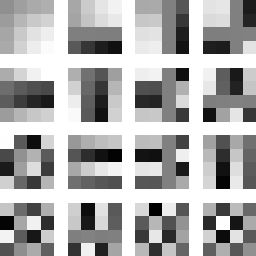
\includegraphics[width=0.15\linewidth]{./figures/mddt_sep_rdot_s4_p02.png}}
	\hfill
	\subfloat[sep. \acs{IPM} 6]
	{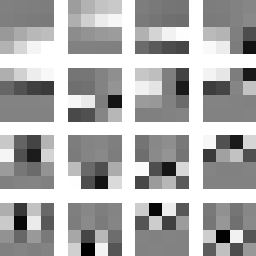
\includegraphics[width=0.15\linewidth]{./figures/mddt_sep_rdot_s4_p06.png}}
	\hfill
	\subfloat[sep. \acs{IPM} 10]
	{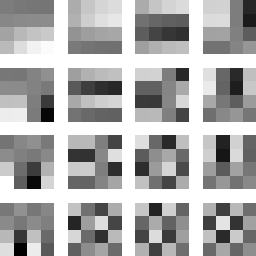
\includegraphics[width=0.15\linewidth]{./figures/mddt_sep_rdot_s4_p10.png}}
	\hfill
	\subfloat[sep. \acs{IPM} 18]
	{
\includegraphics[width=0.15\linewidth]{./figures/mddt_sep_rdot_s4_p18.png}}
	\hfill
	\subfloat[sep. \acs{IPM} 26]
	{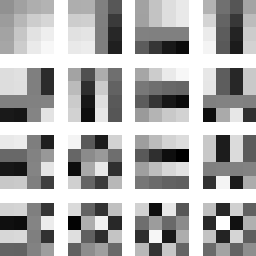
\includegraphics[width=0.15\linewidth]{./figures/mddt_sep_rdot_s4_p26.png}}
	\\
	\subfloat[n-sep. \acs{IPM} 2]
	{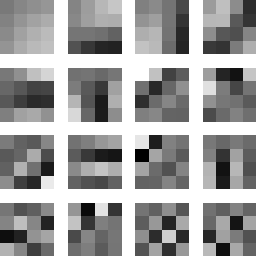
\includegraphics[width=0.15\linewidth]{./figures/mddt_nsep_rdot_s4_p02.png}}
	\hfill
	\subfloat[n-sep. \acs{IPM} 6]
	{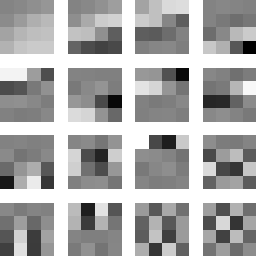
\includegraphics[width=0.15\linewidth]{./figures/mddt_nsep_rdot_s4_p06.png}}
	\hfill
	\subfloat[n-sep. \acs{IPM} 10]
	{
\includegraphics[width=0.15\linewidth]{./figures/mddt_nsep_rdot_s4_p10.png}}
	\hfill
	\subfloat[n-sep. \acs{IPM} 18]
	{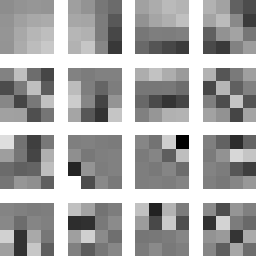
\includegraphics[width=0.15\linewidth]{./figures/mddt_nsep_rdot_s4_p18.png}}
	\hfill
	\subfloat[n-sep. \acs{IPM} 26]
	{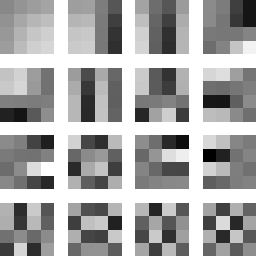
\includegraphics[width=0.15\linewidth]{./figures/mddt_nsep_rdot_s4_p26.png}}
	\caption{$4\times4$ separable and non-separable \acs{RDOT} for different \acsp{IPM}}
	\label{fig:rdot_4x4_bases}
\end{figure}

After having corroborated that the learning has output better performing
transforms in terms of distortion and sparseness, their implementation on top
of \ac{HEVC} is tested and discussed in next section.

\subsection{\acs{MDDT} results on video coding}
\label{sub:mddt_results_on_video_coding}

The \ac{MDDT} systems designed in the previous tested have been using on
\ac{HEVC} using the common test conditions, defined by the
\ac{JCT-VC}~\cite{bossen-12-common-test-conditions}, for \ac{AI} and \ac{RA}
configurations.
The common test conditions consist in encoding each sequence at four different
\ac{QP} points (22, 27, 32, 37) and computing the average bit-rate savings
with regards to \ac{HEVC}.

\subsubsection{Bit-rate savings}
\label{ssub:mddt_bit_rate_savings}

Tables~\ref{tab:mddt_ai} and~\ref{tab:mddt_ra} contain the performances of
different \ac{MDDT} systems for \ac{AI} and \ac{RA} configurations,
respectively, for the different sequence classes of the \ac{HEVC} test set.
The last line of the table represents the average bit-rate savings for all
sequences (it does not correspond to the averaged bit-rate savings per class).

\begin{table}[tb]
	\centering
	\scriptsize
	\begin{tabular}{l|rr|rr|rr|rr|rr|rr}
		\multicolumn{1}{c}{} &
		\multicolumn{4}{c|}{$4\times4$} &
		\multicolumn{4}{c|}{$8\times8$} &
		\multicolumn{4}{c}{$4\times4$ \& $8\times8$} \\
		\cline{2-13}
		\multicolumn{1}{c}{} &
		\multicolumn{2}{c|} {sep} &
		\multicolumn{2}{c|} {non-sep} &
		\multicolumn{2}{c|} {sep} &
		\multicolumn{2}{c|} {non-sep} &
		\multicolumn{2}{c|} {sep} &
		\multicolumn{2}{c} {non-sep} \\
		\hline
		Class & KLT & RDOT & KLT & RDOT & KLT & RDOT & KLT & RDOT & KLT & RDOT & KLT & RDOT \\
		\hline\hline
		A ($2560\times1600$) & 0.1  & 0.1  & -0.2 & -0.2 & -1.0 & -1.0 & -1.6 & -1.6 & -0.9 & -0.9 & -1.6 & -1.6 \\
		B ($1920\times1080$) & -0.1 & -0.2 & -0.5 & -0.8 & -0.4 & -0.8 & -1.5 & -2.5 & -0.4 & -0.9 & -1.6 & -2.8 \\
		C ($832\times480$)   & -0.2 & -0.6 & -1.5 & -2.5 & -0.4 & -0.8 & -2.4 & -4.0 & -0.5 & -1.3 & -3.1 & -5.1 \\
		D ($416\times240$)   & -0.1 & -0.6 & -1.2 & -2.0 & -0.2 & -0.6 & -1.2 & -2.1 & -0.3 & -1.1 & -1.9 & -3.4 \\
		E ($1280\times720$)  & 0.4  & 0.3  & -0.1 & -0.4 & -0.9 & -1.2 & -2.1 & -2.9 & -0.6 & -0.9 & -1.8 & -3.0 \\
		F (various res.)     & 0.1  & -0.8 & -0.6 & -2.0 & 0.1  & -0.2 & -1.1 & -2.4 & 0.3  & -0.9 & -1.2 & -3.5 \\
		\hline\hline           
		Seq. Avg. & 0.0  & -0.3 & -0.7 & -1.3 & -0.5 & -0.7 & -1.6 & -2.6 & -0.4 & -1.0 & -1.9 & -3.2 \\
	\end{tabular}
	\caption{Average bit-rate savings (\%) for each \ac{HEVC} Class in \acs{AI}}
	\label{tab:mddt_ai}
\end{table}

\begin{table}[tb]
	\centering
	\scriptsize
	\begin{tabular}{l|rr|rr|rr|rr|rr|rr}
		\multicolumn{1}{c}{} &
		\multicolumn{4}{c|}{$4\times4$} &
		\multicolumn{4}{c|}{$8\times8$} &
		\multicolumn{4}{c}{$4\times4$ \& $8\times8$} \\
		\cline{2-13}
		\multicolumn{1}{c}{} &
		\multicolumn{2}{c|} {sep} &
		\multicolumn{2}{c|} {non-sep} &
		\multicolumn{2}{c|} {sep} &
		\multicolumn{2}{c|} {non-sep} &
		\multicolumn{2}{c|} {sep} &
		\multicolumn{2}{c} {non-sep} \\
		\hline
		Class & KLT & RDOT & KLT & RDOT & KLT & RDOT & KLT & RDOT & KLT & RDOT & KLT & RDOT \\
		\hline\hline
		A ($2560\times1600$) & 0.0  & 0.1  & 0.0  & -0.1 & -0.3 & -0.4 & -0.7 & -0.8 & -0.3 & -0.4 & -0.7 & -0.9 \\
		B ($1920\times1080$) & 0.0  & -0.1 & -0.3 & -0.5 & -0.2 & -0.5 & -0.9 & -1.4 & -0.2 & -0.6 & -1.0 & -1.6 \\
		C ($832\times480$)   & -0.1 & -0.4 & -0.8 & -1.4 & -0.2 & -0.4 & -1.2 & -2.2 & -0.2 & -0.7 & -1.6 & -2.9 \\
		D ($416\times240$)   & 0.0  & -0.2 & -0.5 & -1.1 & -0.1 & -0.3 & -0.5 & -1.1 & -0.1 & -0.5 & -0.9 & -1.7 \\
		E ($1280\times720$)  & 0.1  & -0.2 & -0.4 & -0.9 & -0.3 & -0.7 & -1.0 & -2.0 & -0.3 & -0.9 & -1.1 & -2.5 \\
		F (various res.)     & 0.1  & -0.6 & -0.3 & -1.3 & 0.1  & -0.1 & -0.5 & -1.4 & 0.2  & -0.7 & -0.6 & -2.2 \\
		\hline\hline
		Seq. Avg. & 0.0  & -0.2 & -0.4 & -0.8 & -0.2 & -0.4 & -0.8 & -1.5 & -0.2 & -0.6 & -1.0 & -1.9 \\
	\end{tabular}
	\caption{Average bit-rate savings (\%) for each \ac{HEVC} Class in \acs{RA}}
	\label{tab:mddt_ra}
\end{table}


The first column of both tables corresponds to the separable \ac{KLT}-based
\ac{MDDT} for $4\times4$ \acp{TU}, which, as demonstrated
in~\cite{jain-75-nearest-neighbors, jain-76-klt-random-process}, corresponds
to using a \ac{DST}.
The average bit-rate savings with regards to \ac{HEVC} for this system are
non-existing \ac{HEVC}, as it already uses the \ac{DST} for those blocks.

The differences between both transform learning approaches (\ac{KLT} and
\ac{RDOT}) can be observed by looking at each pair of columns.
Results are very consistent with what was anticipated in the \ac{RDOT} metric
domain:
the \ac{RDOT}-based \ac{MDDT} outperforms the \ac{KLT} in every case
(separability, \ac{TU} size, class and coding configuration).

It is also worth-noticing the impact of separability:
non-separable configurations provide systematically higher gains than the
separable ones, especially important for those systems involving $8\times8$
\acp{TU}.

For the combined $4\times4$ and $8\times8$ system in \ac{AI} the bit-rate
savings are over 3\% and almost 2\% in \ac{RA}.
The \ac{KLT} systems are about one point below.
The detailed performances of the combined systems are included in
table~\ref{tab:detailed_mddt_bd_rate}.
Despite having used classes B and C for the transform learning, consistent
bit-rate savings are achieved across the whole test set.
Moreover, classes D and E (not included in the learning set) present higher
bit-rate savings than class B.
It is also worth noticing that the \ac{RDOT} systems do not present losses for
any sequence, which is not the case for the \ac{KLT}.

\begin{table}[tb]
	\centering
	\scriptsize
	\begin{tabularx}{\textwidth}{c|X|rr|rr|rr|rr}
		\multicolumn{2}{c}{} &
		\multicolumn{8}{c}{$4\times4$ \& $8\times8$} \\
		\cline{3-10}
		\multicolumn{2}{c}{} &
		\multicolumn{4}{c|}{AI} &
		\multicolumn{4}{c}{RA} \\
		\cline{3-10}
		\multicolumn{2}{c}{} &
		\multicolumn{2}{c|}{sep} &
		\multicolumn{2}{c|}{non-sep} &
		\multicolumn{2}{c|}{sep} &
		\multicolumn{2}{c}{non-sep} \\
		\cline{2-10}
		\multicolumn{1}{c}{} & {Sequence} &
		{KLT} & {RDOT} & {KLT} & {RDOT} &
		{KLT} & {RDOT} & {KLT} & {RDOT} \\
		\hline\hline
		\multirow{5}{0.10\textwidth}{\centering Class A ($2560\times1600$)}
		& NebutaFestival       & -0.5 & -0.4 & -0.7 & -0.4  & -0.1 & -0.1 & -0.1 & -0.1 \\
		& PeopleOnStreet       & -1.2 & -1.3 & -2.5 & -2.5  & -0.5 & -0.5 & -1.1 & -1.1 \\
		& SteamLocomotiveTrain & -0.5 & -0.4 & -0.6 & -0.5  & 0.0  & 0.0  & -0.1 & -0.3 \\
		& Traffic              & -1.3 & -1.5 & -2.7 & -2.9  & -0.6 & -0.9 & -1.5 & -2.0 \\
		\cline{2-10}
		& Average              & -0.9 & -0.9 & -1.6 & -1.6  & -0.3 & -0.4 & -0.7 & -0.9 \\
		\hline\hline
		\multirow{6}{0.10\textwidth}{\centering Class B ($1920\times1080$)}
		& BasketballDrive      & 0.1  & -0.6 & -1.1 & -2.8  & -0.2 & -0.4 & -1.2 & -1.8 \\
		& BQTerrace            & 0.3  & -0.9 & -2.2 & -4.6  & 0.0  & -0.6 & -1.3 & -2.5 \\
		& Cactus               & -0.9 & -1.5 & -2.3 & -3.4  & -0.3 & -0.8 & -1.2 & -2.2 \\
		& Kimono1              & -0.4 & -0.5 & -0.9 & -1.1  & 0.0  & -0.2 & -0.3 & -0.5 \\
		& ParkScene            & -1.2 & -1.3 & -1.7 & -1.9  & -0.6 & -0.7 & -0.9 & -1.2 \\
		\cline{2-10}
		& Average              & -0.4 & -0.9 & -1.6 & -2.8  & -0.2 & -0.6 & -1.0 & -1.6 \\
		\hline\hline
		\multirow{5}{0.10\textwidth}{\centering Class C ($832\times480$)}
		& BasketballDrill      & -1.2 & -1.8 & -7.9 & -11.9 & -0.6 & -0.9 & -3.8 & -6.3 \\
		& BQMall               & 0.0  & -1.1 & -0.8 & -2.6  & 0.1  & -0.6 & -0.3 & -1.5 \\
		& PartyScene           & 0.0  & -1.1 & -1.0 & -2.6  & -0.1 & -0.7 & -0.7 & -1.7 \\
		& RaceHorses           & -0.8 & -1.3 & -2.6 & -3.6  & -0.4 & -0.6 & -1.4 & -2.0 \\
		\cline{2-10}
		& Average              & -0.5 & -1.3 & -3.1 & -5.1  & -0.2 & -0.7 & -1.6 & -2.9 \\
		\hline\hline
		\multirow{5}{0.10\textwidth}{\centering Class D ($416\times240$)}
		& BasketballPass       & -0.1 & -0.9 & -1.5 & -3.1  & -0.1 & -0.5 & -1.0 & -1.8 \\
		& BlowingBubbles       & -0.1 & -1.0 & -1.8 & -3.5  & -0.1 & -0.5 & -0.9 & -1.9 \\
		& BQSquare             & 0.1  & -1.0 & -0.9 & -2.7  & 0.1  & -0.5 & -0.2 & -1.4 \\
		& RaceHorses           & -1.0 & -1.3 & -3.4 & -4.3  & -0.3 & -0.4 & -1.4 & -1.8 \\
		\cline{2-10}
		& Average              & -0.3 & -1.1 & -1.9 & -3.4  & -0.1 & -0.5 & -0.9 & -1.7 \\
		\hline\hline
		\multirow{4}{0.10\textwidth}{\centering Class E ($1280\times720$)}
		& FourPeople           & -1.2 & -1.5 & -2.4 & -3.2  & -0.6 & -1.2 & -1.5 & -2.5 \\
		& Johnny               & -0.3 & -0.7 & -1.5 & -2.8  & -0.1 & -0.8 & -1.0 & -2.4 \\    
		& KristenAndSara       & -0.2 & -0.6 & -1.6 & -3.0  & -0.1 & -0.7 & -0.9 & -2.5 \\
		\cline{2-10}
		& Average              & -0.6 & -0.9 & -1.8 & -3.0  & -0.3 & -0.9 & -1.1 & -2.5 \\
		\hline\hline
		\multirow{5}{0.10\textwidth}{\centering Class F (various resolutions)}
		& BasketDrillText      & -0.8 & -1.8 & -6.1 & -10.0 & -0.5 & -0.9 & -3.1 & -5.6 \\
		& ChinaSpeed           & 0.4  & -0.8 & 0.0  & -1.8  & 0.2  & -0.4 & -0.1 & -1.0 \\
		& SlideEditing         & 0.7  & -0.6 & 1.0  & -0.5  & 0.5  & -0.8 & 0.8  & -0.8 \\
		& SlideShow            & 0.7  & -0.5 & 0.4  & -1.8  & 0.5  & -0.5 & 0.2  & -1.5 \\
		\cline{2-10}
		& Average              & 0.3  & -0.9 & -1.2 & -3.5  & 0.2  & -0.7 & -0.6 & -2.2 \\
		\hline\hline
		All Sequences
		& Overall          & -0.4 & -1.0 & -1.9 & -3.2  & -0.2 & -0.6 & -1.0 & -1.9 \\
	\end{tabularx}
	\caption{Detailed bit-rate savings (\%) for combined $4\times4$ \& $8\times8$
	\acs{MDDT} systems}
	\label{tab:detailed_mddt_bd_rate}
\end{table}

A remarkable point stands out of the test set: the \emph{BasketballDrill}
sequence from class C, with bit-rate savings of almost 12\% using the
non-separable \ac{RDOT} in \ac{AI}.
This is due to the fact that this sequence presents highly directional
patterns that cannot be dealt with separable transforms, as the table
indicates.
Almost all the performance is lost when using separable systems.
For illustrative purposes, figure~\ref{fig:detailed_mddt_bd_rate} represents
graphically the results from table~\ref{tab:detailed_mddt_bd_rate}.

\begin{figure}[tp]
	\centering
	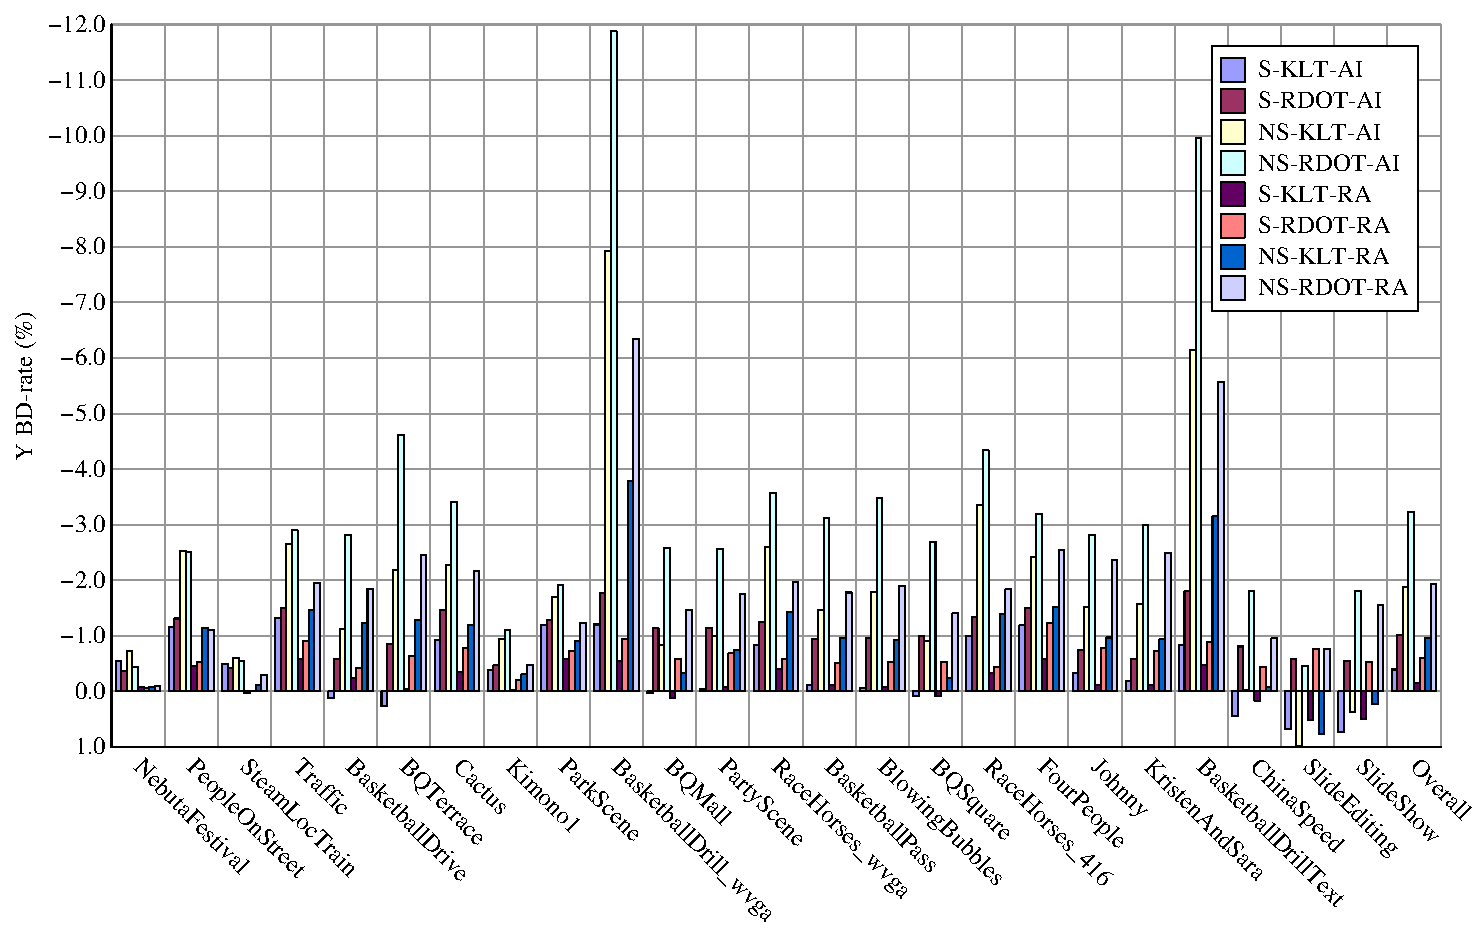
\includegraphics[width=1\linewidth]{./figures/detailed_mddt_4_8.pdf}
	\caption{Bit-rate savings for combined $4\times4$ \& $8\times8$ \acs{MDDT}
	systems}
	\label{fig:detailed_mddt_bd_rate}
\end{figure}

As a final note on the results, all transforms learnt for the presented
\ac{MDDT} systems have used residuals issued from \ac{AI} coding
configurations and have only been enabled for intra coded residuals in
\ac{HEVC}.
Nonetheless, around two thirds of the bit-rate savings achieved for the
\ac{AI} coding configurations have been achieved in \ac{RA}.

A final comment on the designed transforms regarding the scanning of the
transformed coeffients:
the transform base vectors for each \ac{IPM} have been sorted taking into
account the scanning that \ac{HEVC} performs implicitly, illustrated in
figure~\ref{fig:mdcs}.
For non-separable transforms, base vectors can be placed in any order, but
separable transforms does not have this freedom, as such, a scanning matrix is
needed to make sure the transform coefficients are sorted properly.

\subsubsection{Coding complexity}
\label{ssub:mddt_coding_complexity}

Regarding the complexity of the system, the increase in the encoding and
decoding time is only due to the lack of fast algorithms for \acp{KLT} and
\acp{RDOT}.
Due to the way the quad-tree partitioning works in \ac{HEVC}, if, for
instance, a $16\times16$ \ac{TU} provides a better rate-distortion trade-off
than splitting it into $8\times8$ \acp{TU}, the $4\times4$ will not be
explored.
Since the \ac{MDDT} system improves $4\times4$ and $8\times8$ \acp{TU}, it
becomes more likely that a split $16\times16$ \ac{TU} into four $8\times8$
\acp{TU} works better than without splitting.
In that case, the $4\times4$ \acp{TU} will also be explored, which will lead
to an increase in complexity with regards to \ac{HEVC}, since more coding
possibilities are being explored.
Table~\ref{tab:mddt_complexity} summarises the coding complexity for \ac{MDDT}
systems using separable and non-separable transforms for $4\times4$ and
$8\times8$ \acp{TU}.
The complexity for \ac{KLT} and \ac{RDOT} based systems is equivalent, since
transforms are performed as generic matrix multiplications.
For $4\times4$ \acp{TU}, the complexity in both coding and decoding times
remains approximatively the same as that of \ac{HEVC}, however, for bigger
\acp{TU}, the differences due to fast algorithms start becoming more
noticeable.

\begin{table}[tb]
	\centering
	\small
	\begin{tabular}{l|rr|rr|rr}
		& \multicolumn{2}{c|}{$4\times4$}
		& \multicolumn{2}{c|}{$8\times8$}
		& \multicolumn{2}{c}{$4\times4$ \& $8\times8$} \\
		& sep & non-sep & sep & non-sep & sep & non-sep \\
		\hline\hline
		Encoding & 101\% & 102\% & 107\% & 111\% & 108\% & 112\% \\
		Decoding & 101\% & 102\% & 103\% & 105\% & 105\% & 107\% \\
	\end{tabular}
	\caption{Relative average complexity of \acs{MDDT} systems to \acs{HEVC}}
	\label{tab:mddt_complexity}
\end{table}

\subsubsection{\acs{MDDT} storage requirements}
\label{ssub:mddt_storage_requirements}

The transforms used in the \ac{MDDT} system are, in general, not describable
with a mathematical formula in the same way the \ac{DCT} and the \ac{DST} are.
As such, additional memory is required to store these transforms and make them
available to the encoder and the decoder.
Assuming each transform coefficient is quantised to one byte, the storage
requirements for a non-separable transform for $N\times N$ \acp{TU} is:
\begin{equation}
	\acs{ROM}_{\text{non-sep}} =
	N^2 \cdot N^2 \cdot \frac{\unit{1}{\kilo B}}{\unit{1024}{B}} \cdot M
	\label{eqn:rom_nsep}
\end{equation}
The needed \acs{ROM} for separable transforms is:
\begin{equation}
	\acs{ROM}_{\text{sep}} =
	3 \cdot N \cdot N \cdot \frac{\unit{1}{\kilo B}}{\unit{1024}{B}} \cdot M
	\label{eqn:rom_sep}
\end{equation}
Where the number of \acp{IPM} $M$ is 35 for the \ac{MDDT} system.
Sorting the transform base vectors in the proper order is crucial to assist
the entropy coding~\cite{ye-08-intra-directional-scanning-mddt}.
For this reason, there is a factor 3 for the \acs{ROM} requirements in the
separable case: horizontal transform, vertical transform and scanning matrix
for each pair of transforms.
The non-separable transforms do not need a scanning matrix, since the base
vectors can be sorted to output the signal with an appropriate coeffient
order.
Table~\ref{tab:mddt_rom} contains the \acs{ROM} requirements for the \ac{MDDT}
systems in both separable and non-separable designs.
This table illustrates the drawback of using non-separable transforms
regarding the storage.
Even the \ac{MDDT} system using only non-separable transforms for $4\times4$
\acp{TU} needs more \acs{ROM} than the complete separable \ac{MDDT} system.

\begin{table}[tb]
	\centering
	\small
	\begin{tabular}{l|rr|rr|rr}
		& \multicolumn{2}{c|}{$4\times4$}
		& \multicolumn{2}{c|}{$8\times8$}
		& \multicolumn{2}{c}{$4\times4$ \& $8\times8$} \\
		& sep & non-sep & sep & non-sep & sep & non-sep \\
		\hline\hline
		\acs{ROM} (kB) & 1.64 & 8.75 & 6.56 & 140.00 & 8.20 & 148.75 \\
	\end{tabular}
	\caption{Additional \acs{ROM} required to store \acs{MDDT} transforms}
	\label{tab:mddt_rom}
\end{table}

\section{Conclusions}
\label{sec:conclusions}

Transform designs presented in Chapter~\ref{cha:transform_coding}, namely the
\ac{KLT} and the \ac{RDOT}, have been put to the test through the \ac{MDDT}, a
technique for intra coded blocks that consists in designing an adapted
transform per \ac{IPM}.
During the learning phase, the \ac{RDOT} metric has presented coherent results
with the knowledge acquired from literature regarding the \ac{KLT}, \ac{DCT}
and \ac{DST}.
These transforms have been evaluated using the \ac{RDOT} metric and have
corroborated the results obtained in the \ac{BD}-rate domain:
for intra prediction residuals, the \ac{DST}-VII has a better \ac{BD}-rate
score than the \ac{DCT}-II, and so does using the \ac{RDOT} metric.

The designed transforms have been tested in a modified version of \ac{HEVC}
using the \ac{MDDT} technique.
Non-separable transforms present a significant improvement in terms of
bit-rate savings over their separable counterparts.
Moreover, the \ac{RDOT} design approach has provided better results in terms
of \ac{BD}-rate than the \ac{KLT} consistently all over the tested sequences,
with no losses for any of them.
Consequently, the \ac{KLT} will no longer be considered in the upcoming
sections, only \ac{RDOT}-based systems will be designed.

The complexity of the \ac{MDDT} systems remains comparable to that of
\ac{HEVC}, since the default transform is replaced with an adapted one.
Therefore, the increase in complexity is only due to the fact that transforms
are implemented as matrix multiplications due to the lack of fast algorithms.

The following chapter presents an improvement on \ac{MDDT}, which will allow
transforms to be more adapted to intra prediction residuals and provide new
coding alternatives to \ac{HEVC}.

\part{Contributions}
\label{prt:contributions}

\chapter{The mode-dependent transform competition}
\label{cha:the_mode_dependent_transform_competition}
\chaptertoc

\section{Introduction}
\label{sec:introduction_mdtc}

Chapter~\ref{cha:the_mode_dependent_directional_transforms} revisited the
\acf{MDDT} technique, its origins and motivation, and how it was discarded in
the final \ac{HEVC} standard in favour of a more simplified approach.
However, the \ac{MDDT} technique has good potential when used with \acp{RDOT},
especially in their non-separable design.

This Chapter is focused on improving upon the \ac{MDDT} technique by
increasing the number of available transforms.
The main idea is to provide a fixed number of transforms per \acf{IPM} that
will compete against each other in the \ac{RDO} loop, in the same ways as
block sizes and \acp{IPM} do.
This implies that, for a given block size and \ac{IPM}, there will be no
longer a unique transform, but a set of them, and the encoder will choose the
one that provides the best trade-off in terms of rate-distortion.

Transform competition is not an entirely new concept in \ac{HEVC}.
A rudimentary form of competition already exists for $4\times4$ intra
predicted luma residuals:
the choice between using the \ac{DST}-VII and not using a transform at all
already exists.
This behaviour is controlled by the
\texttt{transform\_skip\_flag}~\cite{JCTVC-F077, JCTVC-H0208}.
This flag is activated when transforming a residual does not suppose any
benefit in terms of rate-distortion, which might be due to the fact that the
residuals contains only noise, amongst others.

Early work on transform competition in \ac{HEVC} is detailed
in~\cite{arrufat-14-transform-competition-rdot}, and the actual work in this
Chapter has been published in~\cite{arrufat-15-mdtc}.

\section{Multiple transform design using the \acs{RDOT} metric}
\label{sec:multiple_transform_design}

Since the main purpose of the transforms is to increase the bit-rate savings
in \ac{HEVC}, the design process is carried out accordingly:
the default \ac{HEVC} transforms for $4\times4$ and $8\times8$ blocks (the
\ac{DST} and \ac{DCT}, respectively) are kept and a number of additional
transforms are learnt to capture those residuals \ac{HEVC} transforms are not
adapted to.

The learning set is the same as in
Chapter~\ref{cha:the_mode_dependent_directional_transforms}:
residuals issued from an \ac{AI} \ac{HEVC} coding of classes B and C from the
\ac{HEVC} test set, grouped by \ac{IPM}.
For each \ac{IPM}, $2^N$ transforms are learnt, in addition to the \ac{HEVC}
default transforms.
Algorithm~\ref{alg:clustering} describes how the learning has been carried out
in each \ac{IPM}.
Assuming the desired output are $2^N$ additional transforms, the performed
steps are:
\begin{enumerate}
	\item Initial random classification of the residuals into $1+2^N$ classes.
	\item For the $2^N$ classes that are not assigned to the \ac{HEVC}
		transform, learn a separable or non-separable transform, depending on
		the desired configuration.
	\item Evaluate each residual using the RDOT metric and assign it to the
		transform that minimises the value.
	\item Repeat steps 2 and 3 until convergence.
\end{enumerate}
An example for $N=1\Rightarrow2^N=2$ additional transforms is provided in
figure~\ref{fig:clustering}.

\begin{algorithm}
	\SetKwData{append}{append}
	\SetKwInOut{Input}{input}\SetKwInOut{Output}{output}
	\Input{Residuals $\x$ from a given \acl{IPM}}
	\Output{Set of $2^N$ \acp{RDOT} $A_n$}
	\BlankLine%
	Initial random classification into $1+2^N$ classes
	\BlankLine%
	\While{!convergence}
	{
			\For{$n=1$ \KwTo{} $2^N$}
			{
				Learn a \ac{RDOT} on $\text{Class}_n$
				using~\eqref{eqn:rdot-nsep} or~\eqref{eqn:rdot-sep}, depending
				on separability
			}
			\ForEach{block $\x$}
			{
				\For{$n=0$ \KwTo{} $2^N$}
				{
					$\delta_n =
					{\Vert \x - \A^T_n\c\Vert}^2 + \lambda{\Vert\c\Vert}_0$
				}
				$\displaystyle n^* = \text{arg}\min\limits_n(\delta_n)$\\
				$\text{Class}_{n^*}$.append ($\x$)
			}
	}
	\caption{Multiple transform design}
	\label{alg:clustering}
\end{algorithm}

\begin{figure}[tp]
	\centering
	\includegraphics{./figures/clustering.pdf}
	\caption{Clustering and transform learning for a given set of residuals}
	\label{fig:clustering}
\end{figure}

Figure~\ref{fig:mdtc_rdot_metric_ntransforms} presents the averaged \ac{RDOT}
metric value for all \acp{IPM} residuals when using an increasing number of
transforms for $4\times4$ and $8\times8$ residuals.
The starting point in~\ref{fig:mdtc_rdot_metric_ntransforms}.a
and~\ref{fig:mdtc_rdot_metric_ntransforms}.b corresponds to the \ac{RDOT} metric
evaluated on \ac{HEVC} default transforms, which corresponds to the one shown
in figure~\ref{fig:rdot_metric_learning}, from the previous Chapter.

The \ac{RDOT} metric decreases with the number of transforms, but it can be
seen how it stagnates when the number of transforms is considerably high.

Furthermore, there is an important gap in the \ac{RDOT} metric between
separable and non-separable transform.
For $4\times4$ blocks, the value achieved with separable transforms, is
achieved with half the number of non-separable transforms.
The gap is even more important for $8\times8$ blocks.

\begin{figure}[tb]
	\centering
	\subfloat[\acs{RDOT} metric evolution with the number of $4\times4$
	transforms]
	{\includegraphics{./figures/rdot_ntransforms_4_plot.pdf}}
	\\
	\subfloat[\acs{RDOT} metric evolution with the number of $8\times8$
	transforms]
	{\includegraphics{./figures/rdot_ntransforms_8_plot.pdf}}
	\caption{Average \ac{RDOT} metric evolution for the learning set depending
	on the number of transforms}
	\label{fig:mdtc_rdot_metric_ntransforms}
\end{figure}

\section{Performances of the \acs{MDTC} system}
\label{sec:performances_of_the_mdtc_system}

\begin{figure}[tb]
	\centering
	\subfloat[\acs{BD}-rate evolution with the number of additional $4\times4$
	transforms]
	{\includegraphics{./figures/bdrate_ntransforms_4_plot.pdf}}
	\\
	\subfloat[\acs{BD}-rate evolution with the number additional of $8\times8$
	transforms]
	{\includegraphics{./figures/bdrate_ntransforms_8_plot.pdf}}
	\caption{Average \acs{BD}-rate evolution for the learning set depending
	on the number of transforms}
	\label{fig:mdtc_bdrate_ntransforms}
\end{figure}

This section presents the performances of the \ac{MDTC} systems designed in
the previous section on the full \ac{HEVC} test set.

Figure~\ref{fig:mdtc_bdrate_ntransforms} illustrates how the \ac{BD}-rate for
the \ac{AI} configuration on the \ac{HEVC} test set decreases with the number
of transforms.
The behaviour in the \ac{BD}-rate domain is close to the one observed in the
\ac{RDOT} metric domain in figure~\ref{fig:mdtc_rdot_metric_ntransforms}.

In order to find out the minimum and maximum performances of the designed
\ac{MDTC} systems, two systems have been evaluated on the full \ac{HEVC} test
set in \ac{AI} and \ac{RA} coding configurations, named:
\begin{itemize}
	\item Low complexity system: one additional transform per \ac{IPM}
		for both $4\times4$ and $8\times8$ \acp{TU}.
	\item High performance system: 16 additional transforms per \ac{IPM} for
		$4\times4$ \acp{TU} and 32 for $8\times8$ \acp{TU}.
\end{itemize}
The performances of the low complexity and high performance systems are
summarised in table~\ref{tab:bd_rate_mdtc}.
The first thing to notice is that no losses are observed with regards
\ac{HEVC} in any sequence.
On one hand, the low complexity system is able to achieve average bit-rate savings of
around 3.8\% with non-separable transforms, and around 2.4\% with separable
transforms.
On the other hand, the high complexity system provides average bit-rate
savings of over 4\% for its separable version, and over 7\% for the
non-separable one.
Around two thirds of the gain observed in the \ac{AI} configuration is
obtained in the \ac{RA} coding.

\ac{MDTC} systems overcome the \ac{MDDT} systems by a significant amount,
even in their low complexity configuration, around 1 point of \ac{BD}-rate is
gained.

There are some sequences that stand out, notably the \emph{BasketballDrill},
which already showed high gains using the \ac{MDDT} technique.
This sequence has de particularity of presenting a large amount of directional
patterns, which lead to bit-rate savings of over 25\%.
The \ac{BD}-rate curves for this sequence are presented in
figure~\ref{fig:mdtc_bdrate_basketball_drill}.
For low bit-rates, corresponding to \acp{QP} of 32 and 37, the bitstream size
is almost kept untouched, but the \ac{PSNR} is substantially improved.
For higher bit-rates, the improvements are present in both axis.
\begin{figure}[tb]
	\centering
	\includegraphics{./figures/bdrate_basketballdrill_wvga_plot.pdf}
	\caption{\emph{BasketballDrill} \acs{BD}-rate curves for non-separable
	high performance \acs{MDTC}}
	\label{fig:mdtc_bdrate_basketball_drill}
\end{figure}

The visual improvements are provided in figure~\ref{fig:mdtc_bdrill_visual}.
The first sub-figure displays the original block, which has not been coded
yet, and the two other sub-figures the result of coding that block using
\ac{HEVC} and the non-separable high performance \ac{MDTC}.
The comparison is pertinent, as both sequences have the same bit-rate at
\ac{QP} 37 (around \unit{3.3}{\mega bps}, see
figure~\ref{fig:mdtc_bdrate_basketball_drill}).
It is easy to see the improvements made by the \ac{MDTC} system along the
diagonal patterns of the image:
The lines are cut when coding with \ac{HEVC} but they remain continuous using
\ac{MDTC} thanks to non-separability.

\begin{figure}[tb]
	\centering
	\subfloat[Original crop]
	{\includegraphics[width=0.25\linewidth]{./figures/bdrill_orig_crop.png}}
	\hfill
	\subfloat[\acs{HEVC} at \acs{QP} 37]
	{\includegraphics[width=0.25\linewidth]{./figures/bdrill_hevc_qp37_crop.png}}
	\hfill
	\subfloat[\acs{MDTC} at \acs{QP} 37]
	{\includegraphics[width=0.25\linewidth]{./figures/bdrill_mdtc_qp37_crop.png}}
	\caption{A $100\times100$ block from \emph{BasketballDrill} encoded at
	\acs{QP} 37 with \acs{HEVC} and the non-separable high performance
	\acs{MDTC}}
	\label{fig:mdtc_bdrill_visual}
\end{figure}

\begin{table}[t]
	\centering
	\scriptsize
	\begin{tabularx}{\textwidth}{c|X|rr|rr|rr|rr}
		\multicolumn{2}{c}{} &
		\multicolumn{4}{c|}{$4\times4$: 1+1 --- $8\times8$: 1+1} &
		\multicolumn{4}{c}{$4\times4$: 1+16 --- $8\times8$: 1+32} \\
		\cline{3-10}
		\multicolumn{2}{c}{} &
		\multicolumn{2}{c|}{sep} &
		\multicolumn{2}{c|}{non-sep} &
		\multicolumn{2}{c|}{sep} &
		\multicolumn{2}{c}{non-sep} \\
		\cline{2-10}
		\multicolumn{1}{c}{} & {Sequence} &
		\multicolumn{1}{c}{ \acs{AI}} & \multicolumn{1}{c|}{ \acs{RA}} &
		\multicolumn{1}{c}{ \acs{AI}} & \multicolumn{1}{c|}{ \acs{RA}} &
		\multicolumn{1}{c}{ \acs{AI}} & \multicolumn{1}{c|}{ \acs{RA}} &
		\multicolumn{1}{c}{ \acs{AI}} & \multicolumn{1}{c}{ \acs{RA}} \\
		\hline
		\hline
		\multirow{5}{2cm}{\centering Class A ($2560\times1600$)}
		& NebutaFestival         & -0.3 & -0.1 & -0.5 &  0.0 & -1.1 & -0.1 &  -1.2 &  -0.1 \\
		& PeopleOnStreet         & -1.4 & -0.5 & -2.8 & -1.2 & -4.2 & -1.5 &  -5.7 &  -2.3 \\
		& SteamLocomotiveTrain   & -0.4 &  0.3 & -0.5 & -0.4 & -0.6 &  0.2 &  -0.7 &   0.0 \\
		& Traffic                & -1.7 & -1.3 & -3.1 & -1.7 & -4.5 & -3.7 &  -6.1 &  -5.1 \\
		\cline{2-10} &
		Average                  & -0.9 & -0.4 & -1.7 & -0.9 & -2.6 & -1.3 &  -3.4 &  -1.9 \\
		\hline
		\hline
		\multirow{6}{2cm}{\centering Class B ($1920\times1080$)}
		& BasketballDrive        & -1.2 & -0.4 & -3.2 & -1.8 & -3.2 & -0.7 &  -5.5 &  -2.4 \\
		& BQTerrace              & -1.8 & -1.1 & -5.1 & -2.8 & -4.7 & -2.7 &  -9.2 &  -4.9 \\
		& Cactus                 & -2.0 & -1.2 & -3.8 & -2.4 & -5.2 & -3.1 & -10.9 &  -7.7 \\
		& Kimono1                & -0.5 & -0.3 & -1.1 & -0.5 & -1.1 & -0.8 &  -1.8 &  -1.2 \\
		& ParkScene              & -1.7 & -1.1 & -2.2 & -1.5 & -4.6 & -3.2 &  -5.3 &  -3.7 \\
		\cline{2-10} &
		Average                  & -1.4 & -0.8 & -3.1 & -1.8 & -3.8 &  -2.1&  -6.6 &  -4.0 \\
		\hline
		\hline
		\multirow{5}{2cm}{\centering Class C ($832\times480$)}
		& BasketballDrill        & -2.1 & -1.3 & 12.8 & -7.1 & -5.9 & -3.5 & -25.1 & -14.8 \\
		& BQMall                 & -2.0 & -1.2 & -3.3 & -1.9 & -4.8 & -2.8 &  -6.2 &  -3.6 \\
		& PartyScene             & -2.2 & -1.4 & -3.3 & -2.3 & -4.9 & -3.2 &  -6.2 &  -4.3 \\
		& RaceHorses             & -1.7 & -0.7 & -4.0 & -2.2 & -4.3 & -1.6 &  -6.8 &  -3.2 \\
		\cline{2-10} &
		Average                  & -2.0 & -1.2 & -5.9 & -3.4 & -5.0 & -2.8 & -11.0 &  -6.5 \\
		\hline
		\hline
		\multirow{5}{2cm}{\centering Class D ($416\times240$)}
		& BasketballPass         & -1.7 & -0.8 & -3.7 & -2.0 & -3.9 & -1.8 &  -6.2 & -3.1  \\
		& BlowingBubbles         & -2.0 & -1.2 & -4.2 & -2.4 & -4.3 & -2.7 &  -6.7 & -4.0  \\
		& BQSquare               & -2.3 & -1.2 & -3.7 & -2.0 & -4.6 & -2.7 &  -6.1 & -3.6  \\
		& RaceHorses             & -1.6 & -0.6 & -4.6 & -2.0 & -3.9 & -1.5 &  -7.1 & -3.2  \\
		\cline{2-10} &
		Average                  & -1.9 & -1.0 & -4.1 & -2.1 & -4.2 & -2.2 &  -6.5 & -4.5  \\
		\hline
		\hline
		\multirow{4}{2cm}{\centering Class E ($1280\times720$)}
		& FourPeople             & -1.8 & -1.9 & -3.4 & -3.3 & -4.6 & -5.2 &  -6.2 & -3.1  \\
		& Johnny                 & -1.3 & -1.6 & -3.0 & -2.9 & -3.3 & -4.2 &  -6.7 & -3.o  \\
		& KristenAndSara         & -1.3 & -1.8 & -3.5 & -3.3 & -3.8 & -4.5 &  -6.1 & -3.6  \\
		\cline{2-10} &
		Average                  & -2.0 & -1.8 & -4.2 & -3.2 & -4.7 & -4.4 &  -7.7 & -6.4  \\
		\hline
		\hline
		\multirow{5}{2cm}{\centering Class F (various resolutions)}
		& BasketDrillText        & -2.4 & -1.5 & 11.0 & -6.3 & -6.2 & -3.7 & -21.1 & -13.2 \\
		& ChinaSpeed             & -2.0 & -1.2 & -2.9 & -1.6 & -4.3 & -2.7 &  -4.9 &  -3.0 \\
		& SlideEditing           & -2.0 & -2.2 & -1.8 & -2.0 & -4.8 & -5.1 &  -3.7 &  -4.1 \\
		& SlideShow              & -2.5 & -2.3 & -3.5 & -3.0 & -5.7 & -5.6 &  -6.0 &  -5.9 \\
		\cline{2-10} &
		Average                  & -2.2 & -1.8 & -4.8 & -3.2 & -5.2 & -4.3 &  -9.0 &  -6.5 \\
		\hline
		\hline
		All sequences &
		Overall                  & -1.7 & -1.1 & -3.8 & -2.4 & -4.1 & -2.8 &  -7.1 &  -4.7 \\
	\end{tabularx}
	\caption{Y \acs{BD}-rate (\%) for low complexity and high performance \acs{MDTC} systems}
	\label{tab:bd_rate_mdtc}
\end{table}

\begin{figure}[tb]
	\centering
	\includegraphics[width=1\linewidth]{./figures/mdtc_perf_simple.pdf}
	\caption{\acs{BD}-rate for low complexity \acs{MDTC} system}
	\label{fig:mdtc_perf_simple}
\end{figure}

\begin{figure}[tb]
	\centering
	\includegraphics[width=1\linewidth]{./figures/mdtc_perf_complex.pdf}
	\caption{\acs{BD}-rate for high performance \acs{MDTC} system}
	\label{fig:mdtc_perf_complex}
\end{figure}

\chapter{Incomplete transforms}
\label{cha:incomplete_transforms}

Motivation: try to use non-separable transforms in a simpler way

The previous chapters unveiled notable differences in bit-rate savings when
using separable and non-separable transforms.
Nevertheless, non-separate transforms are really computer costy and unusable
in real life applications.
In this chapter, an approach using non-separable transforms is proposed,
called incomplete transforms.

Reference~\cite{arrufat-15-inc-transforms}

\begin{figure}[tp]
	\centering
	\includegraphics{./figures/inc_tr_diagram.pdf}
	\caption{Illustration of the incomplete transform concepts.
	An additional basis vector ($w_0$ is added to assist an orthogonal
	transform ($v_0,v_1$))}
	\label{fig:inc_tr_diagram}
\end{figure}

\chapter{Realistic system}
\label{cha:realistic_system}
\chaptertoc

Motivation: reduce complexity and ROM

This chapter will take a look at different approaches to simplify the
system presented in
Chapter~\ref{cha:the_mode_dependent_transform_competition} while trying
to degrade its performances as least as possible.

Tears of Steel
\begin{itemize}
	\item $4\times4$ residuals: over 142 million
	\item $8\times8$ residuals: over 343 million
\end{itemize}

\subsection{Main drawbacks}
\label{sub:main_drawbacks}

\begin{itemize}
	\item Testing and learning on almost the same sequences
	\item Encoding time
	\item Decoding time
	\item Storage requirements
\end{itemize}

\section{Non-homogeneous number of transforms per intra prediction mode}
\label{sec:non_homogeneous_number_of_transforms_per_intra_prediction_mode}

Iterations

In order to build the learning set, intra prediction residuals issued from
\ac{HEVC} encodings at four \acp{QP} (22, 27, 32, 37), coming from 59
sequences at different resolutions ($1920\times1080$, $1280\times720$,
$800\times480$) and various frame rates (25, 30, 50, 60, 100, 120, 240
frames per second).

\section{Intra prediction mode symmetries}
\label{sec:intra_prediction_mode_symmetries}

\subsection{Proposals}
\label{sub:proposals}

\begin{itemize}
	\item Usage of separable transforms
	\item Making use of symmetries in prediction modes
	\item Non-homogeneous transform repartition amongst prediction modes
\end{itemize}

\begin{itemize}
	\item Force the number of non-zeroes to 1.
	\item Try to keep good performances from non-separable transforms.
\end{itemize}

\chapter{Discrete trigonometric transforms}
\label{cha:discrete_trigonometric_transforms}

\section{Introduction}
\label{sec:introduction}

\begin{itemize}
	\item Decrease coding complexity $\rightarrow$ fast algorithms.
	\item Reduce the ROM requirements $\rightarrow$ mathematical formula
\end{itemize}

Chapter~\ref{cha:the_mode_dependent_transform_competition} has unveiled the
potential of gains achievable through the \ac{MDTC} technique.
Nevertheless, the presented system had a level of complexity which was to
high to be used in real life applications.
As a result, the following Chapters presented two different approaches to
yield the system less complex.
Chapter~\ref{cha:realistic_system} proposed several ways of reducing the
complexity: taking advantage of the symmetries that might exist within
different \acp{IPM} as well as using a different number of transforms in each
mode.
Chapter~\ref{cha:incomplete_transforms} tried to simplify the system by
designing transforms that make use of only basis vector.
This makes transforming a block less complex than using a regular transform,
even if the incomplete transform is non-separable.
Benefits of this approach are observed on the decoder, being less complex than
that of \ac{HEVC}.

Since the systems presented above have flaws in some aspect, a third approach
is presented in this Chapter to cover them.

\section{The identity as a transform}
\label{sec:the_identity_as_a_transform}

\begin{itemize}
	\item Amongst the \ac{DTT} family, add the identity matrix.
	\item Benefits in terms of computational complexity.
\end{itemize}

\chapter{Perspectives and future work}
\label{cha:perspectives_and_future_work}

\chapter{Publications}
\label{cha:publications}

\section{Non-separable mode dependent transforms for intra coding in HEVC}
\label{sec:non_separable_mode_dependent_transforms_for_intra_coding_in_hevc}

\subsection{Abstract}
\label{sub:mddt_abstract}

Transform coding plays a crucial role in video coders.
Recently, additional transforms based on the \acs{DST} and the \acs{DCT} have
been included in the latest video coding standard, \acs{HEVC}.
Those transforms were introduced after a thoroughly analysis of the video
signal properties.
In this paper, we design additional transforms by using an alternative
learning approach.
The appropriateness of the design over the classical \acs{KLT} learning is
also shown.
Subsequently, the additional designed transforms are applied to the latest
\acs{HEVC} scheme.
Results show that coding performance is improved compared to the standard.
Additional results show that the coding performance can be significantly
further improved by using non-separable transforms.
Bit-rate reductions in the range of 2\% over \acs{HEVC} are achieved with
those proposed transforms.

\section{Rate-distortion optimised transform competition for intra coding in
HEVC}
\label{sec:rate_distortion_optimised_transform_competition_for_intra_coding_in_hevc}

\subsection{Abstract}
\label{sub:tc_abstract}

State of the art video coders are based on prediction and transform coding.
The transform decorrelates the signal to achieve high compression levels.
In this paper we propose improving the performances of the latest video coding
standard, \acs{HEVC}, by adding a set of \acp{RDOT}.
The transform design is based upon a cost function that incorporates a bit
rate constraint.
These new \acp{RDOT} compete against classical \acs{HEVC} transforms in the
\ac{RDO} loop in the same way as prediction modes and block sizes, providing
additional coding possibilities.
Reductions in \acs{BD}-rate of around 2\% are demonstrated when making these
transforms available in \acs{HEVC}.

\section{Mode-dependent transform competition in HEVC}
\label{sec:mode_dependent_transform_competition_in_hevc}

\subsection{Abstract}
\label{sub:mdtc_abstract}

Transform coding plays a key role in state-of-the-art video coders, such as
\acs{HEVC}.
However, transforms used in current solutions do not cover the varieties
of video coding signals.
This work presents an adaptive transform design method that enables the use of
multiple transforms in \acs{HEVC}.
A different transform set is learnt for each intra prediction mode, allowing
the video encoder to perform better decisions regarding block sizes,
prediction modes and transforms.
Different systems are proposed to accommodate trade-offs between complexity
and performance.
Bit rate reductions in the range of 2\% to 7\% are reported, depending on
complexity.

\section{Image coding with incomplete transforms for HEVC}
\label{sec:image_coding_with_incomplete_transforms_for_hevc}

\subsection{Abstract}
\label{sub:it_bstract}

Overcomplete transforms have received considerable attention over the past
years.
However, they often suffer from a complexity burden.
In this paper, a low complexity approach is provided, where an orthonormal
basis is complemented with a set of incomplete transforms: those incomplete
transforms include a reduced number of basis vectors that allow a reduction on
the coding complexity and ensure a certain level of sparsity.
The solution has been implemented in the \acs{HEVC}  standard and compression
gains of around 1\% on average are reported while reducing the decoder
complexity in about 5\%.

\section{Low complexity transform competition for HEVC}
\label{sec:low_complexity_transform_competition_for_hevc}

\subsection{Abstract}
\label{sub:dtt_abstract}

The use of multiple transforms in video coding can lead to substantial
bit-rate savings.
However, these savings come at the expense of increased coding complexity and
storage requirements, which challenge the usability of this approach.
In this paper, a systematic procedure is proposed to design low complexity
systems making use of transform competition.
Multiple trade-offs accommodating the complexity are unveiled and it is
demonstrated that they can keep a certain level of performance.
Compared to the \acs{HEVC} standard, some of them provide bit-rate savings
around 2\% with a 50\% increase in the encoding time, using less than 4 kB of
extra ROM and no added decoding complexity.

\bookmarksetup{startatroot}% to remove Bibliography from the last part
\addtocontents{toc}{\bigskip}% add a separation to the ToC
\backmatter

\bibliographystyle{abbrv} % numbers
%\bibliographystyle{apalike} % Surname et al. 2014
%\bibliographystyle{alpha} % ABC14
\bibliography{refs}

\label{cha:index}
\printindex
\addcontentsline{toc}{chapter}{Index}
\thispagestyle{empty}

\end{document}
